% =====================================================================
%  Beyond Words: Bangla Dialect Identification from Sound and Words
%  Compiler: pdfLaTeX  (Overleaf's default; the fastest to compile)
%  Bibliography: BibTeX (natbib, author-year)
% =====================================================================
\documentclass[12pt,a4paper,oneside]{report}

% ---------- Title-page details: fill these in -------------------------
\newcommand{\thesistitle}{A Neural Network Approach to Classifying Bangla Accentual Diversity}
\newcommand{\thesissubtitle}{Dialect Identification from Sound and from Words}
\newcommand{\thesisauthor}{Towfique Elahe}
\newcommand{\studentid}{183001112}
\newcommand{\thesisauthortwo}{Injamamul Hoque Sikder}
\newcommand{\studentidtwo}{183003012}
\newcommand{\thesisdegree}{Bachelor of Science in Computer Science and Engineering}
\newcommand{\thesisdepartment}{Department of Computer Science and Engineering}
\newcommand{\thesisuniversity}{East Delta University}
\newcommand{\thesissupervisor}{Ashrafur Rahman Chowdhury, Lecturer}
\newcommand{\thesisdate}{November 2026}

% ---------- Fonts (pdfLaTeX) ------------------------------------------
\usepackage[T1]{fontenc}
\usepackage[utf8]{inputenc}
\usepackage{lmodern}

% ---------- Layout ----------------------------------------------------
\usepackage[a4paper,margin=2.5cm,bindingoffset=0.5cm]{geometry}
\usepackage{setspace}
\onehalfspacing
\setlength{\emergencystretch}{1.5em}
\usepackage{titlesec}
\titleformat{\chapter}[display]
  {\normalfont\bfseries\Huge}{\large\MakeUppercase{\chaptertitlename}\ \thechapter}{8pt}{}
\titlespacing*{\chapter}{0pt}{-10pt}{24pt}
\usepackage{fancyhdr}
\pagestyle{fancy}
\fancyhf{}
\fancyhead[L]{\small\nouppercase{\leftmark}}
\fancyhead[R]{\small\thepage}
\renewcommand{\headrulewidth}{0.4pt}
\fancypagestyle{plain}{\fancyhf{}\fancyfoot[C]{\small\thepage}\renewcommand{\headrulewidth}{0pt}}
\setlength{\headheight}{15pt}

% ---------- Content packages ------------------------------------------
\usepackage{amsmath,amssymb}
\usepackage{graphicx}
\graphicspath{{figures/}}
\usepackage{booktabs,tabularx,array,multirow,makecell}
\usepackage{xcolor}
\usepackage[font=small,labelfont=bf,skip=6pt]{caption}
\usepackage{enumitem}
\setlist{itemsep=2pt,topsep=4pt}
\usepackage{float}
\usepackage[round,authoryear]{natbib}
\bibliographystyle{plainnat}
\usepackage[obeyspaces,spaces]{xurl}
\urlstyle{same}
\usepackage[hidelinks,bookmarksnumbered]{hyperref}
\usepackage[nameinlink,capitalise,noabbrev]{cleveref}

% ---------- Helpers ---------------------------------------------------
\newcommand{\fscore}[1]{#1}                       % keeps numbers greppable
\newcommand{\hf}[1]{\path{#1}}                    % model / dataset identifiers
\newcolumntype{L}{>{\raggedright\arraybackslash}X}
\newcommand{\todo}[1]{\textcolor{red}{[TODO: #1]}}

% Bangla words are pre-rendered (figures/src/bangla-words.tex, compiled with
% XeLaTeX) so this document compiles with pdfLaTeX. Usage: \bn{slug}{বাংলা};
% the second argument only keeps the word readable in the source.
\makeatletter
\newcommand{\defbn}[2]{\@namedef{bn@#1}{#2}}
\defbn{mui}{1}\defbn{ami}{2}\defbn{kita}{3}\defbn{ki}{4}\defbn{ai}{5}
\defbn{ar}{6}\defbn{hamar}{7}\defbn{teha}{8}\defbn{biya}{9}\defbn{biye}{10}
\newcommand{\bn}[2]{\raisebox{-4.5pt}{%
  \edef\bn@page{\@nameuse{bn@#1}}%
  
\includegraphics[page=\bn@page]{bangla-words}}}
\makeatother

% If Overleaf still times out, compile one chapter at a time:
% \includeonly{chapters/05-results}

\begin{document}

% ---------- Front matter ----------------------------------------------
\pagenumbering{roman}
\begin{titlepage}
  \centering
  \vspace*{1.5cm}
  {\Large\scshape \thesisuniversity\par}
  \vspace{0.3cm}
  {\large \thesisdepartment\par}
  \vspace{2.5cm}
  {\LARGE\bfseries \thesistitle\par}
  \vspace{0.6cm}
  {\Large \thesissubtitle\par}
  \vspace{2.5cm}
  {\large by\par}
  \vspace{0.3cm}
  {\Large \thesisauthor\par}
  {\normalsize \studentid\par}
  \vspace{2cm}
  {\normalsize A thesis submitted in partial fulfilment of the requirements\\
   for the degree of \thesisdegree\par}
  \vfill
  {\normalsize Supervisor: \thesissupervisor\par}
  \vspace{0.5cm}
  {\large \thesisdate\par}
\end{titlepage}

\chapter*{Declaration}
\addcontentsline{toc}{chapter}{Declaration}

\todo{Replace with your university's required declaration wording.}

I declare that this thesis is my own work and that it has not been submitted for
any other degree or qualification. Where I have used the work of others, it is
acknowledged in the text and listed in the bibliography. Software, datasets and
pretrained models used in this work are cited where they are first used, and the
code that produces every reported number is publicly available.

\todo{If your university requires it, add a statement on the use of AI
assistance in preparing this thesis.}

\vspace{2cm}
\noindent\begin{tabular}{@{}l@{}}
\rule{6cm}{0.4pt}\\
\thesisauthor\\
\thesisdate
\end{tabular}

\chapter*{Abstract}
\addcontentsline{toc}{chapter}{Abstract}

Bangla is spoken in many regional dialects, but automatic dialect identification
for it remains little studied. This thesis classifies 5-second audio clips into
nine classes---eight regional dialects and the standard (Formal) register---using
a 13.1-hour corpus of 9,303 clips collected from television, film and online
media. The corpus has no speaker labels, so the same speaker can appear in both
training and test data; the thesis treats this as a measurement problem rather
than a footnote.

Two routes to dialect identity are compared. The \emph{acoustic route} learns
from the sound alone: hand-crafted MFCC statistics, frozen Whisper-small encoder
embeddings, and an end-to-end fine-tuned XLS-R-300M model reach test macro-F1 of
0.727, 0.917 and 0.952 on a conventional clip-level split. A strict split built
from ECAPA-TDNN pseudo-speaker clusters, calibrated against the known sources of
the Formal clips, lowers these to 0.480, 0.793 and 0.808: 12--14 macro-F1 points
of the pretrained models' clip-level scores came from speaker and channel
overlap. Fine-tuning Whisper-medium and two Bangla-adapted versions of it
raises the strict-split score to 0.92 with a leakage drop of only 6--7 points;
the three are indistinguishable, so Bangla-specific pretraining adds nothing
measurable, while a smaller Bangla FastConformer trails at 0.75.
Channel-suppression augmentation reduces XLS-R's score (0.808 to 0.748), and
frozen Whisper embeddings trained on 10\,\% of the labels outperform MFCC
features trained on all of them.

The \emph{lexical route} transcribes every clip with five off-the-shelf Bangla
speech recognisers and classifies the words. Measured against human
transcripts of dialect speech, the best recogniser---one fine-tuned on regional
speech by its publishers---reproduces 27\,\% of dialect words; recognisers
trained on standard Bangla reproduce 1--4\,\%, rewriting dialect into the
standard form. Matching regional word lists therefore identifies the dialect
poorly (macro-F1 0.36 under the strict split), and a text classifier over the
full transcript reaches 0.63. Combined with the XLS-R model, however, the
words raise the strict-split score from 0.808 to 0.856, and the clip-level score
from 0.952 to 0.967; the clip-level gain is significant, the strict-split gain
borderline.

On clips this short, Bangla dialect identity lies mostly beyond the words: the
acoustic route is the stronger single route, and the lexical route is limited by
speech recognition rather than by classification, yet the two are complementary.
All code, splits and per-clip predictions are released for reproduction.

\vspace{1em}
\noindent\textbf{Keywords:} dialect identification, Bangla, self-supervised
speech models, data leakage, speech recognition, low-resource languages

\chapter*{Acknowledgements}
\addcontentsline{toc}{chapter}{Acknowledgements}

\todo{Write your own acknowledgements. Suggested points are below.}

We thank our supervisor, \thesissupervisor, for their guidance throughout this
project.

The speech corpus was gathered for the studies of Badhon et al.\ (2020) and
Alam et al.\ (2023); this thesis builds on their collection.

This work relies on resources released openly by others: the Bengali.AI
community's OOD-Speech corpus, Ben-10 dataset and speech-recognition models;
the authors of the Vashantor corpus; Hishab, OpenAI and Meta AI for their
pretrained speech models; and the maintainers of PyTorch, Hugging Face
Transformers, SpeechBrain, NVIDIA NeMo and scikit-learn. All GPU computation
used Kaggle's free tier.


\tableofcontents
\listoffigures
\listoftables
% Abbreviations (printed in full by \glsaddall)
\newacronym{did}{DID}{dialect identification}
\newacronym{lid}{LID}{language identification}
\newacronym{asr}{ASR}{automatic speech recognition}
\newacronym{ssl}{SSL}{self-supervised learning}
\newacronym{mfcc}{MFCC}{mel-frequency cepstral coefficients}
\newacronym{mlp}{MLP}{multilayer perceptron}
\newacronym{xlsr}{XLS-R}{cross-lingual speech representations (wav2vec 2.0, multilingual)}
\newacronym{ecapa}{ECAPA-TDNN}{emphasised channel attention, propagation and aggregation time-delay neural network}
\newacronym{ari}{ARI}{adjusted Rand index}
\newacronym{ci}{CI}{confidence interval}
\newacronym{oov}{OOV}{out of vocabulary}
\newacronym{wer}{WER}{word error rate}
\newacronym{cer}{CER}{character error rate}
\newacronym{tfidf}{TF-IDF}{term frequency--inverse document frequency}
\newacronym{ctc}{CTC}{connectionist temporal classification}
\newacronym{scb}{SCB}{standard colloquial Bengali}
\newacronym{cvd}{CVD}{colour-vision deficiency}
\glsaddall


% ---------- Main matter -----------------------------------------------
\cleardoublepage
\pagenumbering{arabic}
\chapter{Introduction}
\label{ch:intro}

\section{Motivation}

Bangla is one language with many voices. A speaker from Sylhet, one from
Chattogram and one from Barishal each speak recognisably differently from one
another and from the standard register heard on national news, in pronunciation,
in rhythm and intonation, and in vocabulary. To a listener from Bangladesh these
differences are often audible within a few seconds. For speech technology they
matter twice: dialect is a source of error for speech recognisers trained on
standard speech, and it is information in its own right, useful for routing
calls, adapting recognisers, or studying language variation at scale.

Automatic \emph{dialect identification} (DID) is the task of predicting a
speaker's dialect from their speech. It sits between language identification,
where the classes are different languages, and speaker identification, where
the classes are individuals \citep{snyder2018xvectors}. For widely studied
languages such as Arabic it has dedicated benchmarks \citep{ali2019mgb5}; for
Bangla it does not. Bangla speech processing is low-resource in general
\citep{bengaliasrsurvey2021}, and previous Bangla dialect work has relied on
hand-crafted acoustic features or on written dialect text
\citep{bengaliaccent2021,bangladial2025}.

Two developments make the task newly tractable. Self-supervised and weakly
supervised speech models---wav2vec~2.0, XLS-R and Whisper
\citep{baevski2020wav2vec,babu2022xlsr,radford2023whisper}---learn general
representations from very large amounts of multilingual audio, including Bangla,
and transfer to new tasks with little labelled data \citep{yang2021superb}. And
public Bangla speech resources have grown: a 1,178-hour corpus of standard
Bangla \citep{rakib2023oodspeech} and, recently, a 78-hour corpus of regional
speech with transcripts \citep{dipto2025ben10}.

\section{Problem statement}

This thesis classifies 5-second audio clips into nine classes: eight regional
dialects (Barishal, Chattogram, Dhaka, Khulna, Mymensingh, Noakhali, Rajshahi,
Sylhet) and the standard register, labelled \emph{Formal}. The corpus contains
9,303 clips, about 13.1 hours, collected from television, film and online media
(\cref{ch:dataset}).

Found data of this kind brings a specific risk. The corpus has no speaker labels,
and for most clips no record of which programme or recording they came from. A
random split can therefore place clips of the same speaker, recorded with the
same microphone in the same room, in both the training and the test set. A model
can then score well by recognising the speaker or the recording channel rather
than the dialect. This is a known failure mode of audio classification on found
data \citep{geirhos2020shortcut,echohawk2026}, but it is usually disclosed as a
caveat rather than measured. Measuring it is a central aim of this thesis.

\section{Two routes to dialect identity}

Dialect is carried by both sound and words. Some cues are acoustic: vowel
quality, consonant realisation, pitch contour and tempo. Others are lexical:
a Barishal speaker may say \bn{mui}{মুই} where standard Bangla has \bn{ami}{আমি} (``I''); a
Sylhet speaker asks \bn{kita}{কিতা} where the standard form is \bn{ki}{কী} (``what'').
The acoustic models used in most of this thesis see only the sound: they consume
log-mel spectrogram frames (Whisper) or the raw waveform (XLS-R) and have no
access to what was said.

The thesis therefore compares two routes:
\begin{itemize}
  \item the \textbf{acoustic route}, which learns dialect from the audio signal
        with hand-crafted features, frozen pretrained embeddings and an
        end-to-end fine-tuned model; and
  \item the \textbf{lexical route}, which transcribes each clip with
        off-the-shelf Bangla speech recognition, separates regional words from
        standard ones, and identifies the dialect from the words.
\end{itemize}
Combining the two answers the question that gives the thesis its title: how much
of Bangla dialect identity is carried by the words, and how much lies beyond
them?

\section{Research questions}

\begin{enumerate}[label=\textbf{RQ\arabic*.}, leftmargin=*]
  \item How accurately can pretrained speech models identify nine Bangla dialect
        classes from 5-second clips, compared with hand-crafted acoustic
        features?
  \item How much of that accuracy comes from speaker and recording-channel
        overlap between training and test data, and do the conclusions survive a
        speaker-disjoint evaluation?
  \item How much dialect information survives off-the-shelf Bangla speech
        recognition, and how well can the dialect be identified from the
        resulting words alone?
  \item Are the acoustic and lexical routes complementary?
\end{enumerate}

\section{Contributions}

\begin{enumerate}
  \item A 9-class, 13.1-hour Bangla dialect corpus pipeline with
        validation, standardisation and leakage-aware splitting, released with
        its exact train/validation/test splits (\cref{ch:dataset,ch:method}).
  \item An application of self-supervised and weakly supervised multilingual
        speech models (Whisper, XLS-R) to Bangla regional dialect
        identification, compared with a hand-crafted baseline under one
        evaluation protocol (\cref{sec:res-clip}).
  \item A measurement of speaker and channel leakage. A strict split built from
        ECAPA-TDNN pseudo-speaker clusters, with its clustering threshold
        calibrated against the known sources of the Formal clips, turns the
        usual ``upper bound'' disclaimer into a measured effect of 12--14
        macro-F1 points for the pretrained models (\cref{sec:res-strict}).
  \item An ablation of representation against split protocol, speaker-group
        bootstrap confidence intervals for every score and gap, and a
        data-efficiency analysis (\cref{sec:res-strict,sec:res-efficiency}).
  \item A negative result: channel-suppression augmentation lowers
        strict-split accuracy, which the thesis attributes to prosody being
        dialect signal rather than nuisance (\cref{sec:res-augment,sec:disc-augment}).
  \item The lexical route: five off-the-shelf Bangla speech recognisers compared
        by how much dialect they preserve, using an automated dialect-word
        recall over 1,666 human-transcribed clips; regional-word matching with
        an interpretable per-region match percentage; a text classifier; and
        acoustic--lexical fusion, which raises the strict-split score from
        0.808 to 0.856 (\cref{sec:res-lexical,sec:disc-words}).
\end{enumerate}

No speech-recognition model was trained or fine-tuned in this work. The only
model trained end to end is the XLS-R dialect classifier; the speech
recognisers are used exactly as their publishers released them.

\section{Thesis outline}

\Cref{ch:background} reviews dialect identification, pretrained speech
representations, Bangla speech resources and evaluation leakage.
\Cref{ch:dataset} describes the corpus. \Cref{ch:method} sets out the splitting
protocols, the acoustic models and the lexical route. \Cref{ch:results} reports
the results, \cref{ch:discussion} interprets them and states the limitations,
and \cref{ch:conclusion} answers the research questions.
\Cref{app:repro,app:settings} give the commands and settings needed to
reproduce every number.

\chapter{Background and Related Work}
\label{ch:background}

This chapter places the thesis in five bodies of work: dialect and accent
identification (\cref{sec:bg-did}); pretrained speech representations
(\cref{sec:bg-ssl}); Bangla speech and dialect resources
(\cref{sec:bg-bangla}); leakage and shortcut learning in evaluation
(\cref{sec:bg-leakage}); and augmentation for speech (\cref{sec:bg-aug}).
\Cref{sec:bg-asr} covers the Bangla speech-recognition work on which the
lexical route builds, and \cref{sec:bg-gap} states the gap this thesis
addresses.

\section{Dialect and accent identification}
\label{sec:bg-did}

Dialect identification is usually framed alongside language identification
(LID) and speaker recognition. Modern systems in all three inherit the embedding
paradigm of x-vectors \citep{snyder2018xvectors}: a network trained to
discriminate classes produces a fixed-length utterance embedding on which a
light classifier operates. The kinship with speaker recognition matters for
this thesis. A representation good at separating speakers is also able to
separate dialect classes by recognising the speakers in them, which is why
speaker overlap between training and test data inflates dialect scores
(\cref{sec:bg-leakage}).

The largest DID benchmarks are for Arabic. The MGB-5 challenge's ADI17 task
asks systems to identify 17 Arabic dialects from broadcast speech
\citep{ali2019mgb5}, the closest analogue to the 9-way Bangla setting here.
\citet{khaled2025arabic} fine-tune a cross-lingual wav2vec~2.0 model on Arabic
dialect audio, the same design as this thesis's fine-tuned model, and
\citet{sullivan2023robustness} show that Arabic DID systems degrade sharply when
moved away from their training conditions. For another lower-resource language,
\citet{hamalainen2021finnish} compare audio and text for Finnish dialect
identification, a precedent for asking whether dialect lives in the sound or in
the words. At larger scale, VoxLingua107 \citep{valk2021voxlingua} builds a
107-language LID corpus from YouTube, illustrating both the power of found data
and its channel confounds, and \citet{kukk2022accented} study how accent
interacts with language identification---relevant to treating the standard
register as a class of its own.

\section{Pretrained speech representations}
\label{sec:bg-ssl}

Wav2vec~2.0 \citep{baevski2020wav2vec} learns speech representations from raw
audio by solving a contrastive task over masked, quantised latent features, and
is then fine-tuned for a downstream task. XLS-R \citep{babu2022xlsr} scales the
same objective to 436,000 hours of speech in 128 languages, Bangla included; its
300-million-parameter variant is the model fine-tuned in this thesis. Whisper
\citep{radford2023whisper} takes a different route: an encoder--decoder
Transformer trained with weak supervision on 680,000 hours of transcribed,
multilingual web audio. Its encoder consumes 80-channel log-mel spectrograms
through two convolutional layers and a Transformer stack; this thesis uses the
encoder of Whisper-small as a frozen feature extractor.

The SUPERB benchmark \citep{yang2021superb} showed that frozen self-supervised
representations with light task heads transfer well across many speech tasks,
which motivates the frozen-embedding baseline here. Probing work on accent
identification \citep{yang2023accent} shows that fine-tuning a wav2vec~2.0
model for accent reshapes how its layers encode prosody---external support for
this thesis's explanation of why pitch and tempo augmentation hurt dialect
identification (\cref{sec:disc-augment}). The pseudo-speaker clustering in
\cref{ch:method} uses ECAPA-TDNN speaker embeddings \citep{desplanques2020ecapa}.

\section{Bangla speech and dialect resources}
\label{sec:bg-bangla}

Bangla speech processing is widely described as low-resource despite the
language's size and dialectal diversity \citep{bengaliasrsurvey2021}. The
closest prior work to the first version of this project classifies Bengali
accents from hand-crafted acoustic features with classical and neural
classifiers \citep{badhon2020accent}, and \citet{alam2023accent} classify Bangla
accent variation from audio with deep neural networks. The corpus used in this
thesis was gathered for those two studies (\cref{ch:dataset}). Text-based Bangla dialect classification
has progressed further: on the BanglaDial dataset, transformer models such as
BanglaBERT reach a reported score of about 89\,\% when classifying written
dialect text from 11 regions \citep{bangladial2025}. That result is a precedent for the lexical
route, with one difference: its text is written by people, whereas the lexical
route in this thesis has to obtain its text from speech recognition.

Regional speech datasets are appearing: a five-region speech dataset
\citep{bdregionalspeech}, the BRADS and BRWDS audio-and-text collections
\citep{brads2025}, and the Ben-10 and RegSpeech12 corpora discussed in
\cref{sec:bg-asr}. Large-scale standard Bangla speech is available in the
crowdsourced Bengali Common Voice corpus \citep{alam2022commonvoice} and in
OOD-Speech \citep{rakib2023oodspeech}.

\section{Leakage, shortcuts and honest evaluation}
\label{sec:bg-leakage}

Deep networks exploit whatever regularity separates the training classes,
including regularities that are not the intended signal
\citep{geirhos2020shortcut}. In audio, recording channel, background and session
are such shortcuts. SpurAudio \citep{spuraudio2026} benchmarks shortcut learning
in audio classification directly, and EchoHawk \citep{echohawk2026} shows, for
acoustic drone detection, that clips sharing a recording session share their
channel and background, and that session-disjoint evaluation collapses inflated
scores---the same phenomenon this thesis measures for dialects. A survey of
audio-classification practice finds evaluation protocols frequently
under-specified \citep{leakage2025iciis}. Together these legitimise reporting the
drop from a clip-level to a group-disjoint split as a finding in itself.

\section{Augmentation for speech}
\label{sec:bg-aug}

Speed and tempo perturbation is a standard and beneficial augmentation in speech
recognition \citep{ko2015augmentation}, where the target transcript does not
depend on prosody. SpecAugment \citep{park2019specaugment} masks time and
frequency bands of the spectrogram and is the canonical feature-level method.
\Cref{sec:res-augment} shows that the analogous waveform-level transforms reduce
dialect-identification accuracy, and \cref{sec:disc-augment} argues why the
recognition intuition does not carry over.

\section{Bangla speech recognition and dialect speech}
\label{sec:bg-asr}

The lexical route depends on three recent resources.

\paragraph{OOD-Speech.} \citet{rakib2023oodspeech} released 1,178 hours of
crowd-read standard Bangla from 22,645 speakers, with a 23-hour test set drawn
from 17 out-of-distribution domains. It was the training data of the 2023
Bengali.AI speech-recognition competition \citep{bengaliai2023competition},
whose winning entry---a fine-tuned Whisper-medium released as
\hf{bengaliAI/tugstugi_bengaliai-asr_whisper-medium} and referred to here as
\emph{Tugstugi}---is one of this thesis's recognisers. Its training transcripts
supply the standard-Bangla vocabulary in \cref{sec:method-lexical}.

\paragraph{Ben-10.} \citet{dipto2025ben10} introduce Ben-10, 78 hours of mostly
spontaneous speech from 394 speakers in ten districts, transcribed in the
dialect as spoken, and benchmark seven speech-recognition systems on it. Word
error rates range from 1.13 for zero-shot Whisper-large-v3 and 1.03 for
Google's cloud recogniser, through 0.87 for Hishab's Conformer and 0.81 for
Tugstugi, to 0.70 for Tugstugi fine-tuned on Ben-10. In a manual analysis of
about 50 dialect words per district, the authors find that the
standard-trained Tugstugi model reproduces 1--9\,\% of dialect words, against
16--53\,\% after fine-tuning on Ben-10, and describe a full-scale analysis as beyond their scope.
The paper is a speech-recognition benchmark, not a dialect-identification
study: it trains no classifier and reports no accuracy. In this thesis its
models serve as transcription front-ends, and its manual dialect-recall
analysis is repeated automatically over its full validation set
(\cref{sec:res-asr}).

\paragraph{Parallel dialect text.} Vashantor \citep{faria2023vashantor}
provides 32,500 sentence pairs translating regional Bangla from Chittagong,
Noakhali, Sylhet, Barishal and Mymensingh into standard Bangla. Because each
pair contains both forms, a regional word can be defined as one that appears on
the dialect side but not on the standard side. RegSpeech12
\citep{hassan2025regspeech12}, from the same group as Ben-10, extends coverage to
twelve dialects, and BanglaDialecto \citep{bangladialecto2024} provides Noakhali
speech with dialect and standard transcriptions; neither is used here, but both
would extend word lists to more of this corpus's classes.

The other recognisers used are Hishab's FastConformer \citep{nandi2023hishab},
trained on about 18,000 hours of mostly broadcast-news Bangla, Whisper-large-v3
\citep{radford2023whisper}, and a public wav2vec~2.0 XLS-R model fine-tuned for
Bangla \citep{arijitx2022wav2vec2}, which stands in for the benchmark's
``Wav2Vec2 (SCB)'' system whose checkpoint is not public.

\section{The gap}
\label{sec:bg-gap}

Prior Bangla dialect work uses either hand-crafted acoustic features on small
corpora or human-written dialect text. None applies pretrained speech models
under an evaluation that controls speaker and channel leakage, and none asks how
much dialect information survives the step from speech to text. This thesis
addresses both: it compares pretrained and hand-crafted acoustic
representations under a measured, leakage-aware protocol, and it tests whether
the words that speech recognition recovers can identify the dialect, alone or in
combination with the sound.

\chapter{Dataset}
\label{ch:dataset}

\section{Source and composition}

The corpus consists of short clips of Bangla speech cut from television shows,
films and online video, originally distributed as MP4 and grouped into one
folder per class. It contains nine classes: eight regional dialects named after
the district or division they are associated with, and the standard register,
labelled Formal (\cref{tab:classes}). After validation, 9,303 clips totalling
about 13.1 hours are usable; two duplicate \path{.ogg} files in the Formal
folder are excluded. Class sizes range from 750 (Khulna) to 1,652 (Formal).

\begin{table}[ht]
  \centering
  \caption{Classes and clip counts, with the number of test clips under the two
  split protocols of \cref{sec:method-splits}.}
  \label{tab:classes}
  \begin{tabular}{lrrr}
    \toprule
    Class & Clips & Test (clip-level) & Test (strict) \\
    \midrule
    Barishal   & 1,257 & 179 & 251 \\
    Chattogram &   797 & 114 & 114 \\
    Dhaka      &   763 & 109 & 103 \\
    Formal     & 1,652 & 236 & 236 \\
    Khulna     &   750 & 107 &  67 \\
    Mymensingh & 1,053 & 151 & 150 \\
    Noakhali   & 1,213 & 174 & 173 \\
    Rajshahi   &   860 & 122 & 110 \\
    Sylhet     &   958 & 137 & 123 \\
    \midrule
    Total      & 9,303 & 1,329 & 1,327 \\
    \bottomrule
  \end{tabular}
\end{table}

\section{Audio properties}

Every clip is standardised to 16\,kHz, mono, 16-bit PCM WAV
(\path{build_manifest.py}). Clips are nominally five seconds long: the median
duration is 5.0\,s and the mean 5.08\,s, but 1,067 clips fall outside
4.5--5.5\,s, with a range of 1.1--8.0\,s; Formal clips are slightly longer
(median 5.6\,s). Five seconds is enough for a listener to recognise many
dialects but excludes longer-range cues such as discourse markers and phrase-level
intonation. Because the material is broadcast and online media, recording
conditions vary widely within and across classes, from studio news to
outdoor drama scenes.

\section{The Formal class}

Formal is a speech register---the standard, prescribed Bangla of news reading
and formal speech---rather than a region. It is kept as a ninth class
deliberately. Distinguishing regionally marked speech from the standard register
is of practical interest in its own right, and Formal is the only class with
recoverable provenance, which makes it the calibration anchor for the strict
split (\cref{sec:method-splits}). A consequence is that the class boundary is
partly one of register: Formal speakers may come from any region, and some
regional clips contain stretches of near-standard speech.

\section{Metadata and the leakage problem}
\label{sec:data-metadata}

The corpus ships no speaker labels and almost no provenance. Regional clips have
sequential filenames (\path{khl271.wav}, \path{shlt479.wav}) that say
nothing about speaker or source. Only the Formal class carries recoverable
source identifiers: 557 of its 1,652 clips embed a YouTube video identifier in
the filename, from 35 distinct videos. For the remaining 8,746 clips---94\,\% of
the corpus---nothing prevents clips of the same speaker, or from the same
programme and recording channel, from appearing on both sides of a random
train/test split. \Cref{sec:method-splits} describes how the thesis estimates
pseudo-speaker groups to control this, and \cref{sec:res-strict} measures its
effect.

The clips were collected from films and dramas as well as from news and
interviews, so some speakers may be actors performing a dialect rather than
native speakers of it. This cannot be checked from the metadata and is listed
among the limitations (\cref{sec:disc-limits}).

\section{External resources for the lexical route}
\label{sec:data-external}

The lexical route (\cref{sec:method-lexical}) uses three public text and speech
resources in addition to the corpus. None contributes training audio to any
dialect classifier.

\begin{description}
  \item[OOD-Speech] \citep{rakib2023oodspeech}: the 963,636 training sentences
    of standard Bangla, distributed with the 2023 Bengali.AI competition
    \citep{bengaliai2023competition}, define the standard-Bangla vocabulary.
  \item[Ben-10] \citep{dipto2025ben10}: the district-labelled dialect
    transcripts of its training set (13,342 clips) contribute regional words for
    the three districts it shares with this corpus (Barishal, Chattogram,
    Sylhet); its public validation set (1,666 clips with audio and human
    transcripts) is the reference for measuring speech-recognition quality.
    Released under CC0.
  \item[Vashantor] \citep{faria2023vashantor}: regional--standard sentence
    pairs for Chittagong, Noakhali, Sylhet, Barishal and Mymensingh contribute
    regional words for those five classes. Released under CC BY 4.0.
\end{description}

\chapter{Methodology}
\label{ch:method}

\section{Task formulation}

Dialect identification is posed as 9-way single-label classification: given a
clip of about five seconds, predict one of Barishal, Chattogram, Dhaka, Formal,
Khulna, Mymensingh, Noakhali, Rajshahi or Sylhet. The headline metric is
macro-averaged F1 on the test split, which weights every class equally despite
the imbalance in \cref{tab:classes}; chance level is about 0.11. Every model is
evaluated under the two split protocols of \cref{sec:method-splits}, and every
headline number carries a bootstrap confidence interval
(\cref{sec:method-eval}).

\Cref{fig:pipeline} shows the two routes compared in this thesis. The acoustic
route (\cref{sec:method-acoustic}) classifies the audio directly; the lexical
route (\cref{sec:method-lexical}) transcribes it first and classifies the words.
Both share the splits, the metric and the evaluation code, and their outputs are
combined by late fusion.

\begin{figure}[ht]
  \centering
  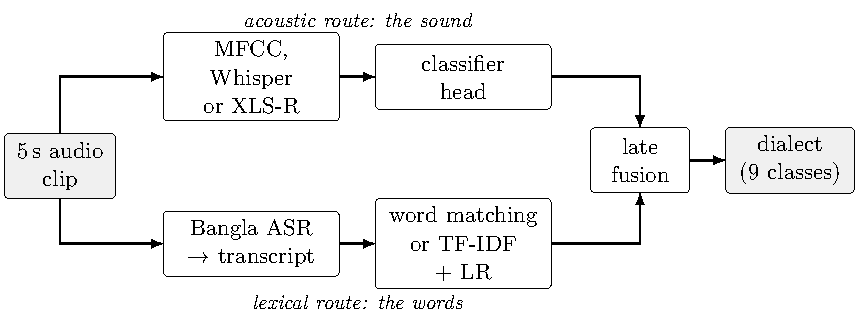
\includegraphics{pipeline}  % source: figures/src/pipeline.tex
  \caption{The two routes to dialect identity. The acoustic route sees only the
  signal; the lexical route sees only the words recovered by speech recognition.
  Each produces class probabilities, which late fusion combines
  (\cref{eq:fusion}).}
  \label{fig:pipeline}
\end{figure}

\section{Splitting protocols}
\label{sec:method-splits}

Two protocols are used throughout (\cref{tab:splits}).

\paragraph{Clip-level split.} \path{build_split.py} draws a stratified
75/10/15 train/validation/test split with seed 42. Clips with a known source
(the 557 sourced Formal clips) are split source-disjointly with
\path{StratifiedGroupKFold}; all other clips are split individually. Because
the same speaker or recording can then appear on both sides, scores under this
protocol are an \emph{upper bound}. The split is committed to the repository
for reproducibility.

\paragraph{Strict pseudo-speaker split.} Each clip is embedded with the
SpeechBrain ECAPA-TDNN speaker model \citep{desplanques2020ecapa}
(\hf{speechbrain/spkrec-ecapa-voxceleb}, 192 dimensions). Within each class the
embeddings are clustered by agglomerative clustering with cosine distance and
average linkage, with no preset number of clusters. The distance threshold is
not hand-picked: it is \emph{calibrated on the Formal class}, whose true sources
are known for 557 clips, by sweeping 0.30--0.90 and keeping the threshold that
maximises the adjusted Rand index \citep{hubert1985ari} between clusters and
true sources. The best threshold is 0.50, with ARI 0.347. Clustering every
class at this threshold yields 1,683 pseudo-speaker groups, and a grouped split
then guarantees that no group crosses train, validation and test (verified: 0
of 1,683).

The modest calibration ARI is acknowledged: pseudo-speakers only partly recover
true sources, so the strict split removes much, but not provably all, of the
speaker and channel overlap. It stands in for true speaker labels, which the
corpus lacks. Formal is not a clean control either: only its 557 sourced clips
are source-disjoint under both protocols, while its other 1,095 clips move from
clip-level splitting to pseudo-speaker grouping like the regional classes.

\begin{table}[ht]
  \centering
  \caption{Split sizes. Per-class test sizes are in \cref{tab:classes}.}
  \label{tab:splits}
  \begin{tabular}{lrrrl}
    \toprule
    Protocol & Train & Validation & Test & Grouping \\
    \midrule
    Clip-level & 6,977 & 997 & 1,329 & sourced Formal clips only \\
    Strict     & 6,931 & 1,045 & 1,327 & 1,683 pseudo-speaker groups \\
    \bottomrule
  \end{tabular}
\end{table}

\section{Acoustic models}
\label{sec:method-acoustic}

All acoustic models share one protocol: inverse-frequency class-weighted
cross-entropy, model selection by validation macro-F1, and seed 42. Models
(a)--(c) are the original comparison; (d) and (e) were added after a
supervisor review, to place Bangla-pretrained encoders beside the multilingual
ones and to fine-tune Whisper as XLS-R was fine-tuned.

\paragraph{(a) MFCC statistics + MLP} (\path{baseline_mfcc.py}). Forty
MFCCs with their first and second differences are mean- and standard-deviation
pooled over time into a 240-dimensional vector, fed to the same head as (b).
This re-implements the spirit of the project's original hand-crafted pipeline
under the current protocol, so that representations are compared fairly.

\paragraph{(b) Frozen Whisper-small + MLP} (\path{baseline_whisper.py}).
Each clip is encoded once by the frozen encoder of \hf{openai/whisper-small};
hidden states are mean-pooled to 768 dimensions and cached. The classifier is a
two-hidden-layer MLP (768--256--256--9, ReLU, dropout 0.3) trained with AdamW
\citep{loshchilov2019adamw} (learning rate $10^{-3}$, weight decay $10^{-4}$)
for 60 full-batch epochs on CPU, which makes it bit-reproducible, keeping the
checkpoint with the best validation macro-F1.

\paragraph{(c) Fine-tuned XLS-R-300M} (\path{finetune_xlsr.py}).
\hf{facebook/wav2vec2-xls-r-300m} with a sequence-classification head; the
convolutional feature encoder is frozen and the Transformer and head are
fine-tuned. Two learning-rate groups (encoder $2\times10^{-5}$, head
$10^{-4}$), 10\,\% linear warm-up then linear decay, batch 8 with gradient
accumulation 2 (effective batch 16), fp16 mixed precision, gradient clipping at
1.0, 20 epochs. Inputs are 5\,s waveforms, padded or trimmed and normalised per
utterance. An 8-epoch pilot (macro-F1 0.865, still rising at the last epoch)
showed that the schedule needed lengthening; at 20 epochs validation plateaus
from about epoch 11 (\cref{fig:training-curve}).

\paragraph{(d) Fine-tuned Whisper-medium encoders} (\path{finetune_xlsr.py --model ...}).
The same recipe as (c), applied to the encoder of three Whisper-medium
checkpoints: \hf{openai/whisper-medium} (multilingual), and the two Bangla
speech-recognition models of \cref{tab:asr-fronts} that share its architecture,
\emph{Tugstugi} (fine-tuned on standard Bangla by Bengali.AI) and \emph{Tugstugi
(Ben-10)} (further fine-tuned on dialect speech). Each is loaded as an
encoder-only classifier: the seq2seq checkpoint's decoder is dropped, and a
projector, mean-pooling over time and a linear classifier are added, mirroring
the XLS-R head (\texttt{WhisperForAudioClassification} in Transformers). Whisper's
encoder is built for 30\,s of input; to train on 5\,s clips at a sixth of the
cost, only the first 250 rows of its (frozen) positional table are kept, which
corresponds to 500 log-mel frames, and the two convolutional input layers are
frozen as XLS-R's feature encoder is. All 24 Transformer layers (302M
parameters) and the head are trained with the hyperparameters of (c), for 12
epochs rather than 20 because XLS-R's validation curve had plateaued by epoch
11 and the larger encoder converges faster; a run takes about 70 minutes on a
T4. Raw amplitude is fed to Whisper's own log-mel front end; the per-utterance
normalisation of (c) is not applied.

\paragraph{(e) Fine-tuned FastConformer} (\path{finetune_xlsr.py --family nemo}).
Hishab's Bangla FastConformer (\hf{hishab/hishab_bn_fastconformer}, NVIDIA NeMo)
is the Bangla-pretrained counterpart of (d) from a different architecture. Its
mel front end and Conformer encoder are taken from the released ASR model, the
encoder output is mean-pooled over the unpadded frames and a linear classifier
is added. The encoder and head are trained with the hyperparameters of (c) for
20 epochs; the encoder is much smaller than Whisper-medium's.

\paragraph{Frozen rows for (d)} (\path{baseline_whisper.py cache --model ...}).
To separate the effect of fine-tuning from that of the encoder, the frozen
recipe of (b) is also run on the Whisper-medium and Tugstugi (Ben-10)
encoders, so that the same checkpoint appears both frozen and fine-tuned.

\paragraph{Augmentation variant} (\path{finetune_xlsr.py --augment}). A
train-only waveform augmentation chain aimed at recording-channel signatures:
gain $\pm 6$\,dB ($p=0.5$), Gaussian noise at 10--30\,dB SNR ($p=0.5$),
seven-band parametric equalisation $\pm 6$\,dB ($p=0.3$), telephone-style
band-pass 300--3400\,Hz ($p=0.15$), pitch shift $\pm 2$ semitones ($p=0.25$),
and time stretch 0.9--1.1 ($p=0.25$).

\section{Evaluation and statistical uncertainty}
\label{sec:method-eval}

Every headline number is one seed on one test set. To separate signal from
sampling noise, \path{bootstrap_ci.py} resamples the saved test predictions
$B = 2{,}000$ times in two ways: resampling clips, and resampling whole
pseudo-speaker or source groups. The group bootstrap is the honest choice,
because clips of one speaker are correlated and a clip bootstrap understates
the variance \citep{efron1993bootstrap}. For each model it reports the 95\,\%
percentile interval of macro-F1, and for each pair of models the interval of
the difference and the proportion of resamples in which the difference is zero
or negative. The clip-level test set contains 565 groups and the strict test
set 230.

\section{Data-efficiency protocol}
\label{sec:method-efficiency}

\path{data_efficiency.py} retrains the MLP head of (a) and (b) on stratified
fractions of 10, 25, 50, 75 and 100\,\% of the training split, three seeds per
point, under both protocols; evaluation is always on the full, fixed test split.
Fine-tuning is excluded because each point would cost a full GPU run.

\section{The lexical route}
\label{sec:method-lexical}

The acoustic models never observe \emph{what} is said. The lexical route asks
how much dialect identity is recoverable from the words alone and whether it
adds to the acoustics. It reuses the splits, the metric and the bootstrap
unchanged, so every number is directly comparable with
\cref{sec:method-acoustic}.

\subsection{Transcription}

The corpus has no transcripts, so text is produced by off-the-shelf Bangla
speech recognition (\path{transcribe.py}). The recognisers follow the Ben-10
benchmark \citep{dipto2025ben10} as far as public checkpoints allow
(\cref{tab:asr-fronts}). \textbf{None was trained or fine-tuned in this work};
each is used as released. Google's paid recogniser and the benchmark's
Ben-10-fine-tuned wav2vec~2.0, which has no public checkpoint, are omitted.

\begin{table}[ht]
  \centering
  \caption{Speech-recognition front-ends. ``Training data'' is as stated by
  the publishers.}
  \label{tab:asr-fronts}
  \small
  \begin{tabularx}{\textwidth}{@{}lL>{\raggedright\arraybackslash}p{3.3cm}@{}}
    \toprule
    Front-end & Checkpoint & Training data \\
    \midrule
    Tugstugi (Ben-10) & \hf{bengaliAI/tugstugi_bengaliai-regional-asr_whisper-medium} & OOD-Speech, then Ben-10 dialect speech \\
    Tugstugi & \hf{bengaliAI/tugstugi_bengaliai-asr_whisper-medium} & OOD-Speech (standard Bangla) \\
    Hishab FastConformer & \hf{hishab/hishab_bn_fastconformer} & $\approx$18k\,h, mostly news \\
    wav2vec2 Bengali\textsuperscript{*} & \hf{arijitx/wav2vec2-xls-r-300m-bengali} & standard Bangla \\
    Whisper-large-v3 & \hf{openai/whisper-large-v3} & multilingual web audio (zero-shot) \\
    \bottomrule
    \multicolumn{3}{@{}l}{\footnotesize\textsuperscript{*}Stand-in for the benchmark's ``Wav2Vec2 (SCB)'', whose checkpoint is not public.}
  \end{tabularx}
\end{table}

Decoding is greedy throughout. For the Whisper models, the language and task
are fixed to Bangla transcription with no prompt and a cap of 128 new tokens on
the 5\,s thesis clips (median output 53 tokens; 0.2\,\% of clips reach 120) and
440 on Ben-10's up-to-30\,s clips; the
two Tugstugi checkpoints ship without a language-token table, so the generation
configuration of the base \hf{openai/whisper-medium} is substituted, which
changes no weights. The wav2vec~2.0 model is decoded by CTC argmax
\citep{graves2006ctc} without a language model; the FastConformer is run through
NVIDIA NeMo \citep{kuchaiev2019nemo}. All 9,303 clips were transcribed on a
Kaggle T4 GPU (43, 45, 82, 15 and 7 minutes for the five front-ends in the
order of \cref{tab:asr-fronts}). A 450-clip pilot run on an Apple M1 agreed with
the T4 output on 93.6\,\% of clips; all reported numbers use the T4
transcripts.

\subsection{Normalisation and the standard-Bangla vocabulary}

All text---transcripts, reference corpora and word lists---passes one tokeniser
(\path{text_utils.py}): Unicode NFC normalisation, Bangla-letter tokens only
(digits, punctuation and Latin script are dropped), word-level normalisation with
\path{bnunicodenormalizer}, and removal of zero-width joiners.

The \emph{standard vocabulary} $V$ is the word inventory of OOD-Speech's
963,636 training sentences \citep{rakib2023oodspeech}: 8.19 million tokens and
156,643 word types, of which the 88,262 types occurring at least three times are
kept to exclude typos. A transcript word outside $V$ is a \emph{candidate
regional word}. The Ben-10 paper characterises its districts by the same
out-of-vocabulary construction.

\subsection{Regional lexicons}

A lexicon maps each region $r$ to a set of words $w$ with a weight
$p(r \mid w)$. With $c_r(w)$ the count of $w$ in region $r$'s text, $N_r$ the
total number of tokens in that text, and add-$\tfrac12$ smoothing,
\begin{equation}
  p(r \mid w) = \frac{(c_r(w) + \tfrac12)/N_r}{\sum_{q} (c_q(w) + \tfrac12)/N_q},
  \label{eq:lexicon-weight}
\end{equation}
so that a word shared by several dialects counts less towards each. Two
lexicons are built (\path{build_lexicon.py}):
\begin{itemize}
  \item The \textbf{external lexicon} comes from human-written dialect text
        independent of the corpus: the Ben-10 training transcripts and the
        regional side of Vashantor (\cref{sec:data-external}). A Vashantor word
        that also appears on the standard side of the same sentence pair is not
        counted as regional. Districts are matched by exact name only, so the
        external lexicon covers Barishal, Chattogram, Sylhet, Noakhali and
        Mymensingh.
  \item The \textbf{in-domain lexicon} comes from the speech-recognition
        transcripts of the \emph{training split only}---verified in code: no
        validation or test clip contributes. A candidate regional word is kept
        for a class if it occurs at least three times across at least two
        pseudo-speakers of that class, which suppresses recognition noise and
        programme-specific words. It covers all classes and is built separately
        for each front-end and each split protocol.
\end{itemize}

\subsection{Classifiers}

Three classifiers operate on the transcripts (\path{lexical_did.py}).

\paragraph{Word matching.} For a clip with tokens $t_1, \dots, t_n$, the
\emph{non-formal share} is $f = \frac{1}{n}\sum_i \mathbb{1}[t_i \notin V]$, and
the \emph{match percentage} for each region is
\begin{equation}
  s_r = \frac{1}{n} \sum_{i=1}^{n} p(r \mid t_i),
  \label{eq:match}
\end{equation}
where $p(r \mid t_i) = 0$ for words absent from region $r$'s lexicon. A clip
with $f < \tau$, or with $s_r = 0$ for every region, is classified as Formal;
otherwise it is assigned to $\arg\max_r s_r$. The threshold $\tau$ is chosen on
the validation split. The method needs no training, and the per-word evidence
behind each decision can be shown to a user.

\paragraph{TF-IDF + logistic regression.} The normalised transcript is
represented by TF-IDF features over word 1--2-grams and character 2--5-grams
(sublinear term frequency, minimum document frequency 2), and classified by
logistic regression with balanced class weights, with the regularisation
strength $C \in \{0.3, 1, 3, 10, 30\}$ chosen on validation
\citep{pedregosa2011sklearn}. Unlike word matching, it uses standard words too.

\paragraph{Late fusion.} With $p_\text{a}$ the class probabilities of the
fine-tuned XLS-R model and $p_\text{l}$ those of the TF-IDF model,
\begin{equation}
  \hat{y} = \arg\max_{c}\; \alpha \log p_\text{a}(c) + (1 - \alpha) \log p_\text{l}(c),
  \label{eq:fusion}
\end{equation}
with $\alpha \in \{0, 0.05, \dots, 1\}$ chosen on validation. XLS-R
probabilities are computed from the Phase~2 and Phase~3 checkpoints on the same
5\,s inputs used in training; their arg\,max reproduces the saved test
predictions exactly on the strict split and on 1,328 of 1,329 clip-level clips,
the one difference coming from M1 versus T4 arithmetic.

\subsection{Speech-recognition reference evaluation}
\label{sec:method-ben10}

The corpus has no reference transcripts, so recognition quality is measured on
Ben-10's public validation set (1,666 clips from ten districts,
\path{ben10_eval.py}). Besides corpus-level word and character error rates on
normalised tokens \citep{jiwer}, \emph{dialect-word recall} is the proportion of
reference tokens outside $V$ that the hypothesis reproduces exactly (counts
matched per clip). It is the full-set, automated counterpart of the Ben-10
paper's hand-counted dialect recall over about 50 words per district.
\emph{Formal-word recall} is the same measure for reference tokens inside $V$.
On the corpus itself, which has no references, the share of transcript tokens
outside $V$ per class is reported for each front-end.

\section{Compute and reproducibility}

Development and all experiments except fine-tuning and transcription ran on an
Apple M1 laptop (16\,GB, PyTorch MPS backend). Fine-tuning ran on Kaggle's free
T4 GPU tier: about 2.5 hours per XLS-R run, 55--75 minutes per Phase 6 run
(about 9 hours for the eight), and about 4.5 hours in all for the lexical
route's transcription. The pipeline survived a mid-project hardware change (GTX 1660 Ti to
M1) with the frozen-embedding baseline reproducing within 0.3 macro-F1 points.
The code uses PyTorch \citep{paszke2019pytorch}, Hugging Face Transformers
\citep{wolf2020transformers}, SpeechBrain \citep{ravanelli2021speechbrain},
librosa \citep{mcfee2015librosa} and scikit-learn \citep{pedregosa2011sklearn}.
\Cref{app:repro} maps every reported number to the command that produces it.

\chapter{Results}
\label{ch:results}

All numbers are test macro-F1 unless stated otherwise. Artifacts are in
\texttt{reports/} of the code repository.

\section{Clip-level results}
\label{sec:res-clip}

On the canonical clip-level split, frozen Whisper-small embeddings with an MLP
head reach a macro-F1 of \fscore{0.917} (accuracy 0.916, $n = 1{,}329$), and
end-to-end fine-tuned XLS-R-300M reaches \fscore{0.952}, 3.5 points higher.
The MFCC baseline reaches \fscore{0.727}. \Cref{tab:clip-perclass} and
\cref{fig:perclass-clip} give the per-class scores.

\begin{table}[ht]
  \centering
  \caption{Per-class test F1, clip-level split (upper bound).}
  \label{tab:clip-perclass}
  \begin{tabular}{lccc}
    \toprule
    Class & MFCC + MLP & Frozen Whisper + MLP & Fine-tuned XLS-R \\
    \midrule
    Khulna     & 0.879 & 0.986 & 0.986 \\
    Sylhet     & 0.873 & 0.951 & 0.982 \\
    Rajshahi   & 0.781 & 0.947 & 0.980 \\
    Formal     & 0.770 & 0.970 & 0.973 \\
    Dhaka      & 0.655 & 0.913 & 0.972 \\
    Barishal   & 0.653 & 0.871 & 0.927 \\
    Chattogram & 0.597 & 0.880 & 0.924 \\
    Mymensingh & 0.651 & 0.890 & 0.912 \\
    Noakhali   & 0.688 & 0.848 & 0.910 \\
    \midrule
    Macro      & \textbf{0.727} & \textbf{0.917} & \textbf{0.952} \\
    \bottomrule
  \end{tabular}
\end{table}

\begin{figure}[ht]
  \centering
  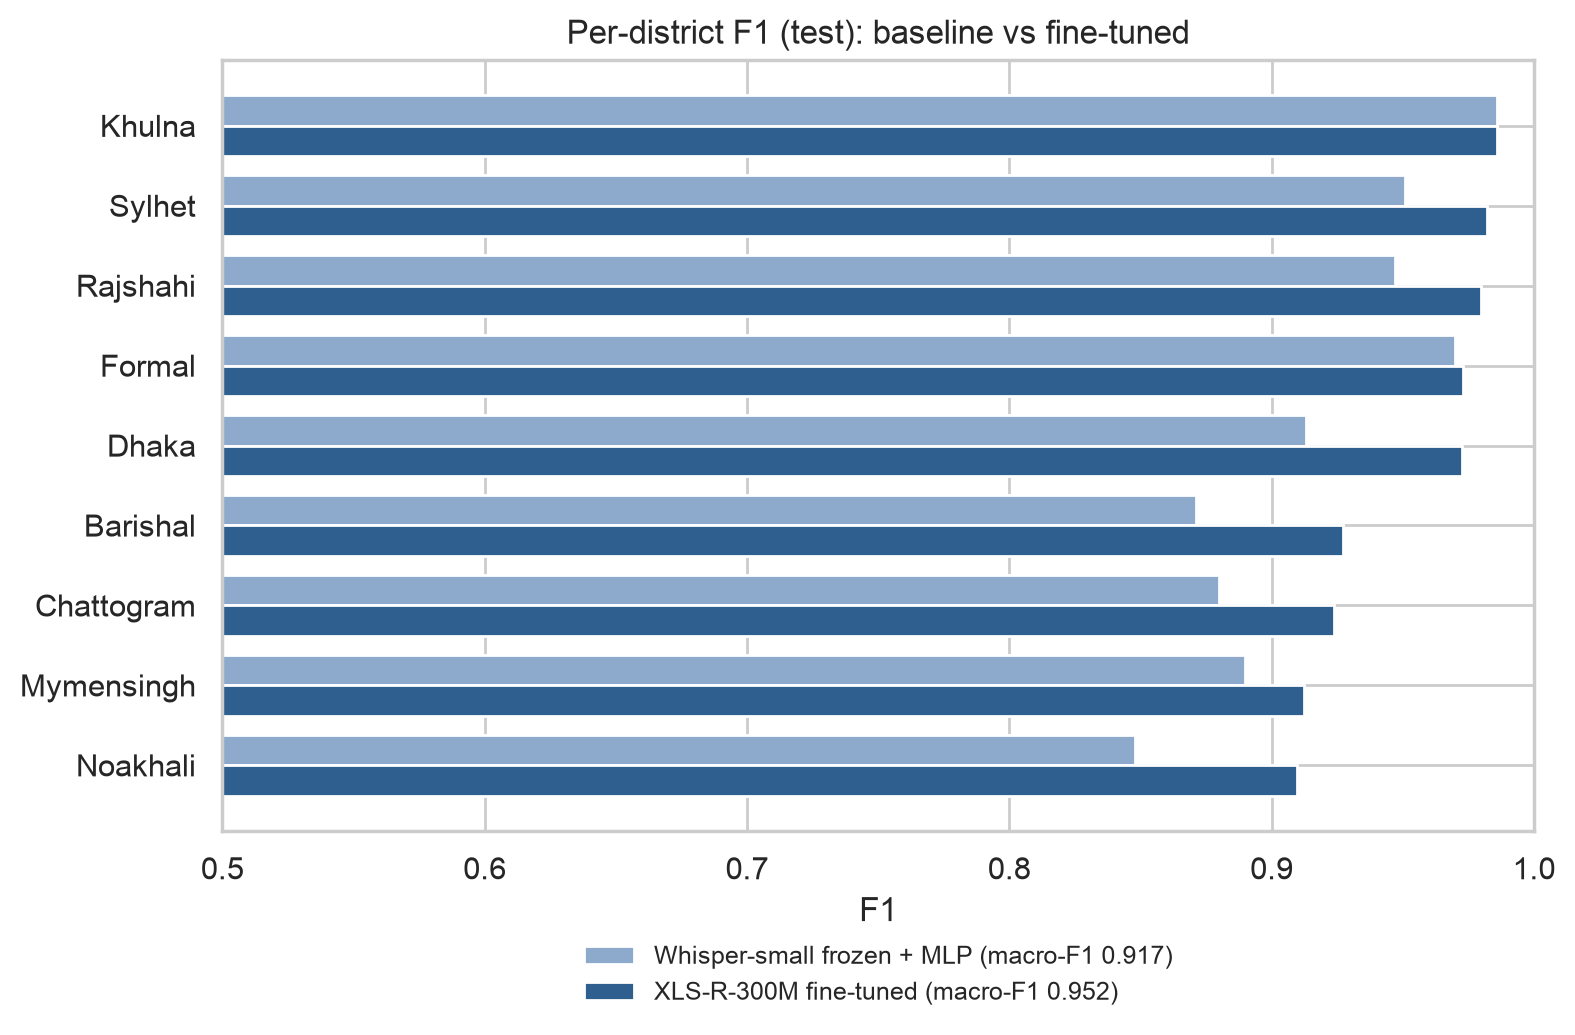
\includegraphics[width=0.85\textwidth]{per_class_f1_comparison.png}
  \caption{Per-class test F1 on the clip-level split: frozen Whisper-small with
  an MLP head against fine-tuned XLS-R-300M.}
  \label{fig:perclass-clip}
\end{figure}

Three observations follow.
\begin{itemize}
  \item Fine-tuning's gains concentrate on the frozen baseline's weakest classes:
        Noakhali (+6.1 points), Dhaka (+5.9), Barishal (+5.6) and Chattogram
        (+4.4). Task adaptation moves capacity towards the hard, acoustically
        close dialects.
  \item The dominant confusion is between Barishal and Noakhali, two southern
        coastal dialects (\cref{fig:confusion}). Fine-tuning halves it, from 31
        to 15 test errors, but does not remove it. Mymensingh, a transitional
        dialect zone, spreads its errors across its neighbours. Errors follow
        dialect geography rather than falling at random.
  \item Training converges: the 8-epoch pilot reached 0.865 and was still
        rising, while the 20-epoch run's validation score plateaus at about 0.95
        from epoch 11 (\cref{fig:training-curve}).
\end{itemize}

\begin{figure}[ht]
  \centering
  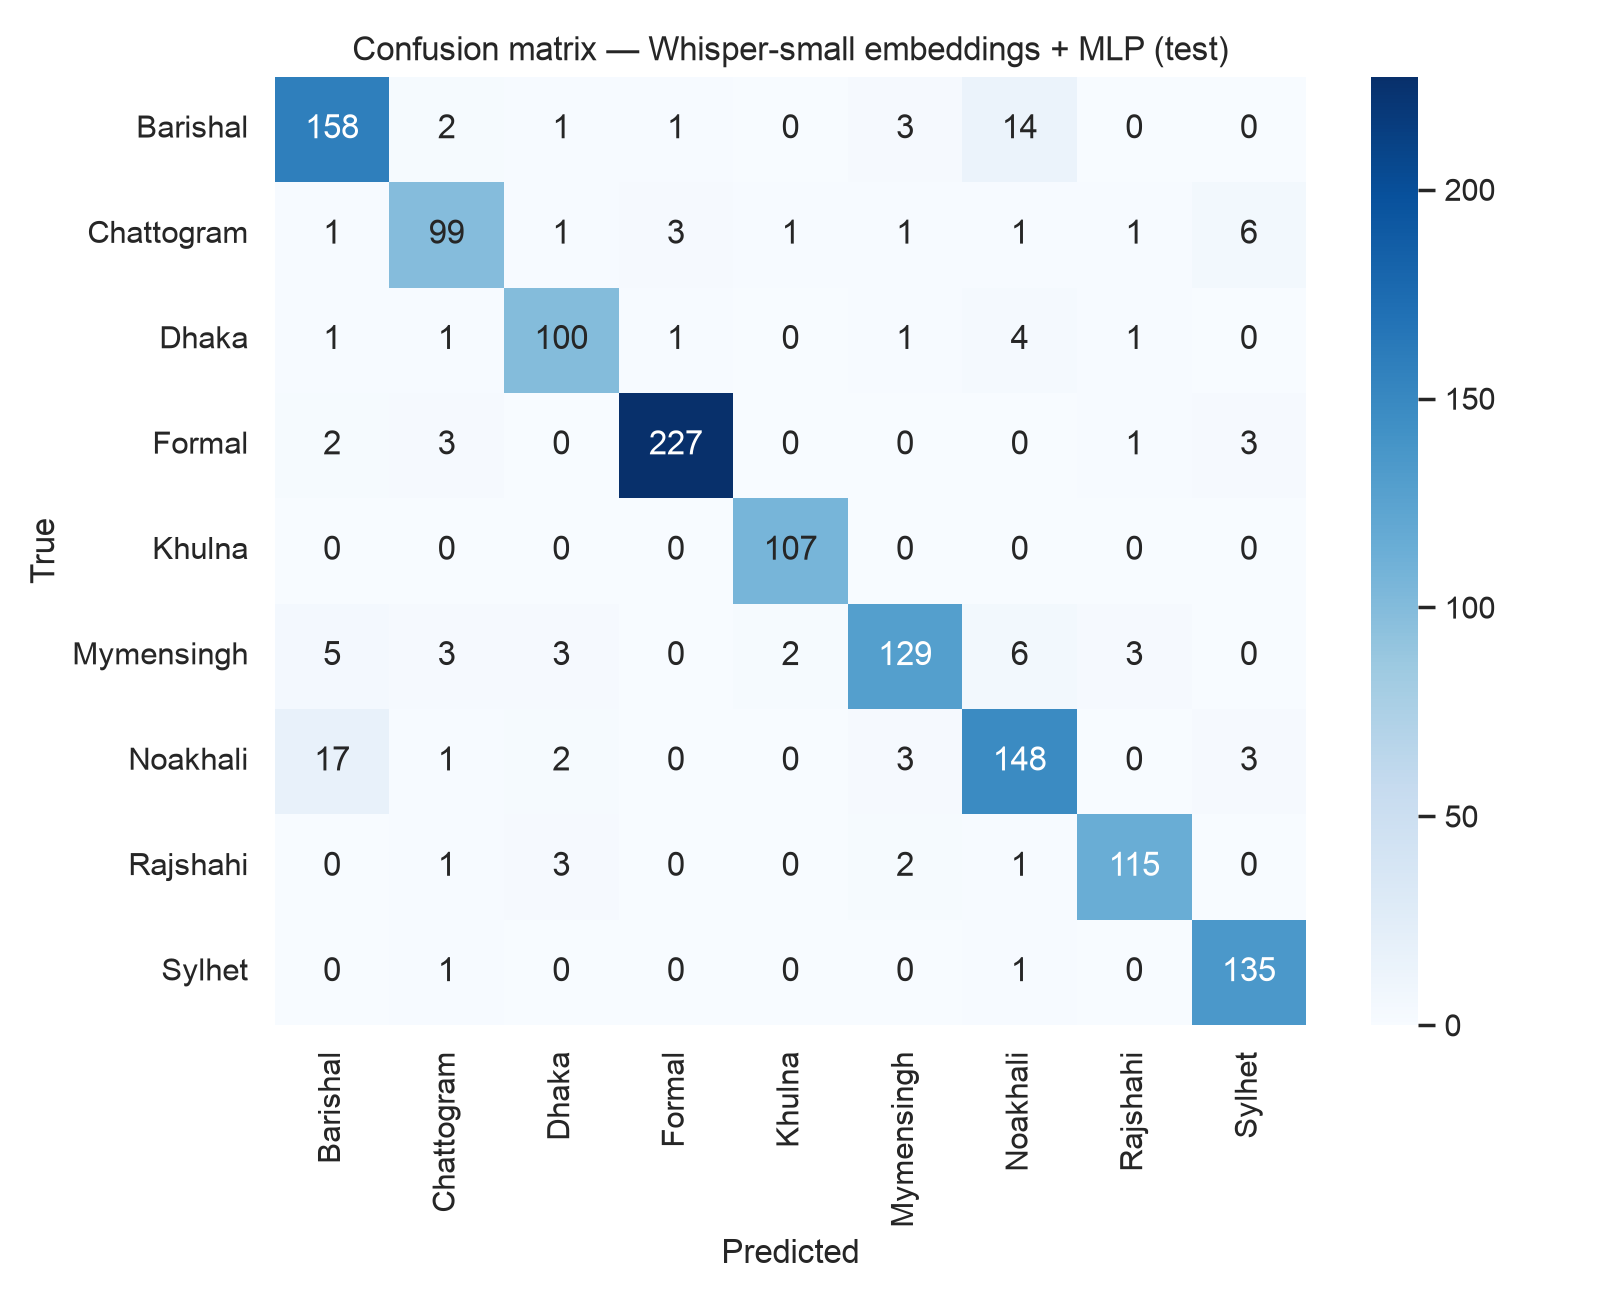
\includegraphics[width=0.64\textwidth]{confusion_matrix_baseline.png}\\[4pt]
  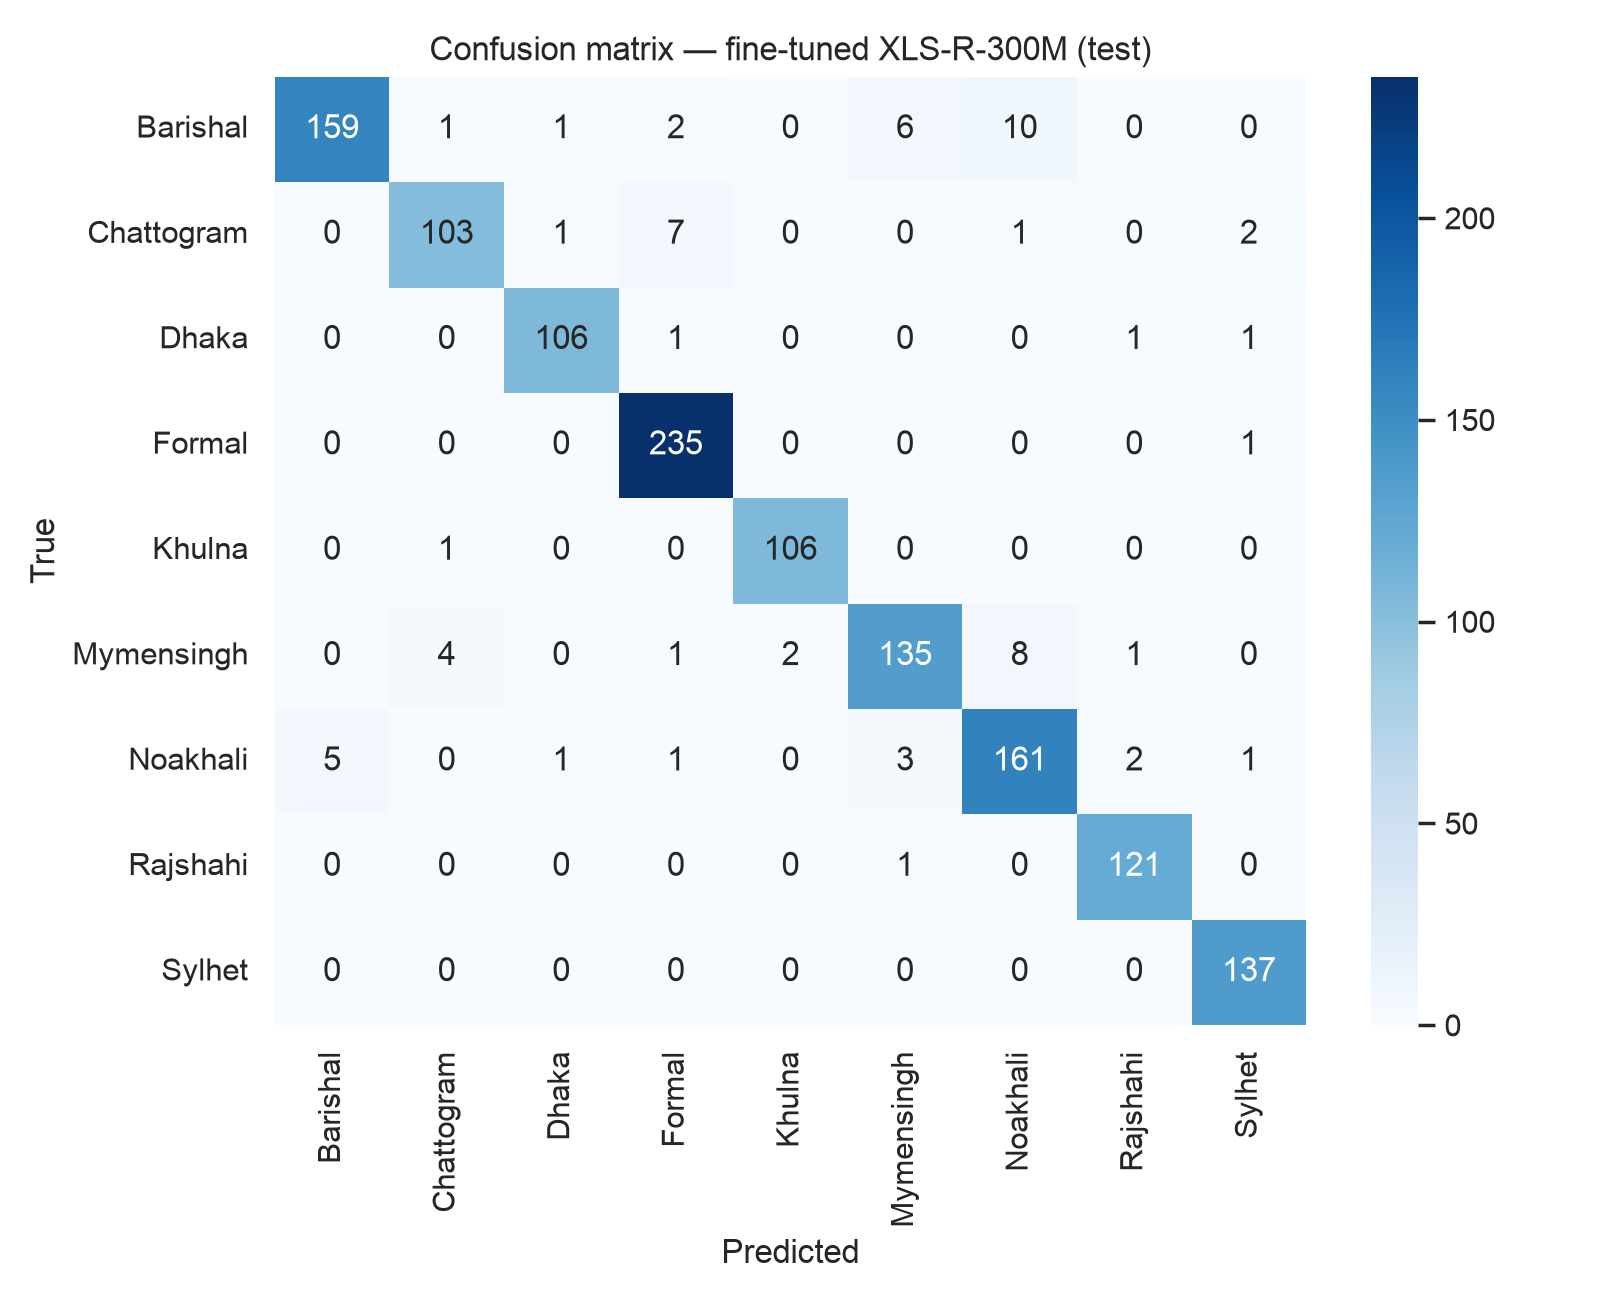
\includegraphics[width=0.64\textwidth]{confusion_matrix_xlsr.png}
  \caption{Test confusion matrices on the clip-level split. Top: frozen
  Whisper-small with an MLP head. Bottom: fine-tuned XLS-R-300M. Rows are true
  classes, columns predictions. The Barishal--Noakhali confusion falls from
  $14 + 17 = 31$ to $10 + 5 = 15$ errors.}
  \label{fig:confusion}
\end{figure}

\begin{figure}[ht]
  \centering
  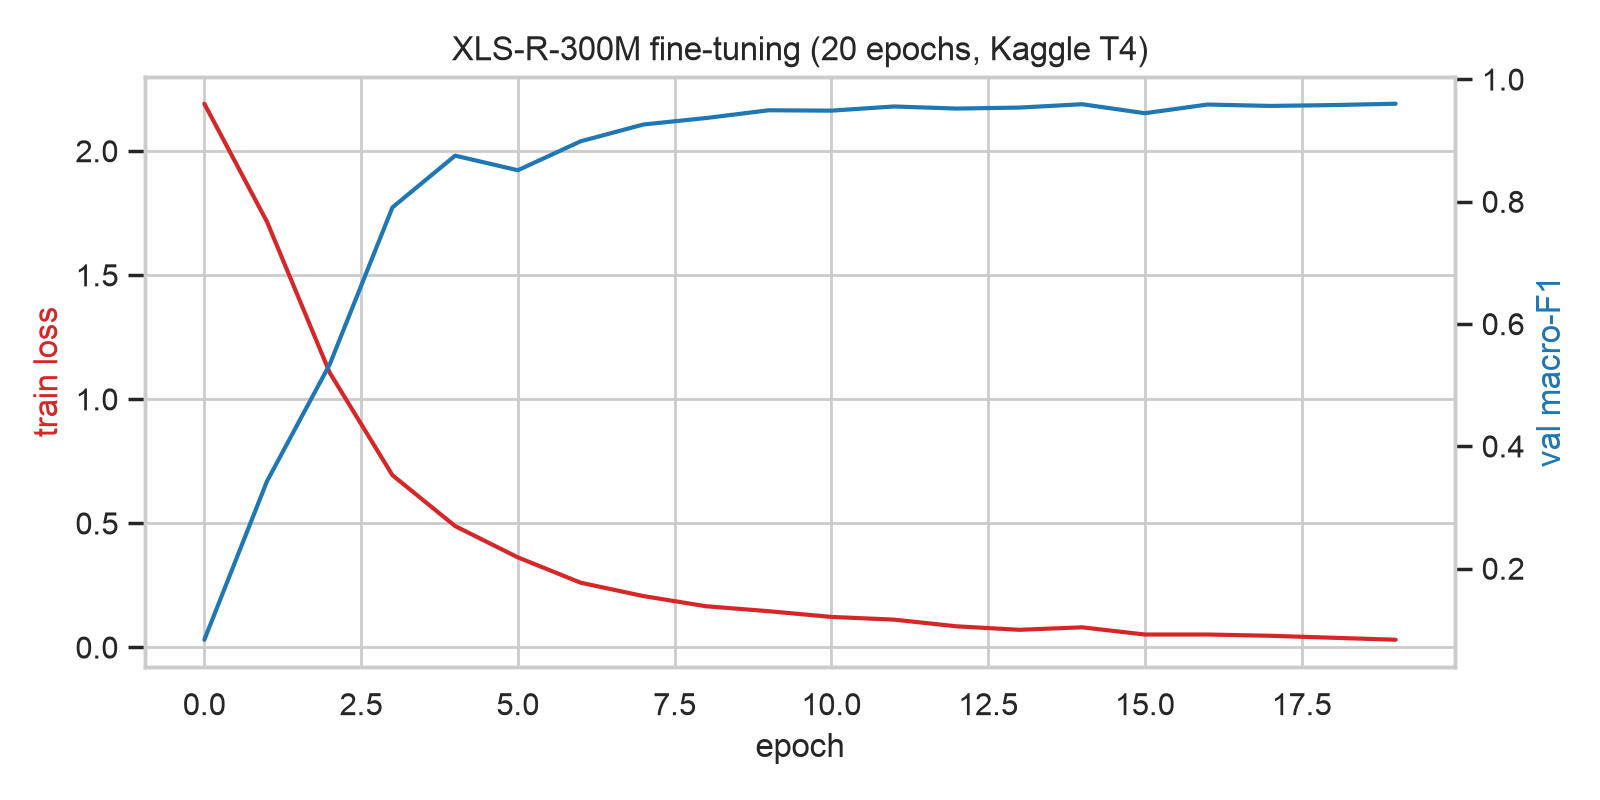
\includegraphics[width=0.85\textwidth]{training_curve_xlsr.png}
  \caption{XLS-R-300M fine-tuning on the clip-level split: training loss (red,
  left axis) and validation macro-F1 (blue, right axis) over 20 epochs on a
  Kaggle T4.}
  \label{fig:training-curve}
\end{figure}

\Cref{fig:tsne} projects frozen Whisper embeddings into two dimensions with t-SNE \citep{vandermaaten2008tsne}. Formal, Sylhet, Rajshahi and
Khulna form recognisable regions even before any task-specific training, while
Barishal, Noakhali and Mymensingh overlap heavily---the same classes the
classifiers confuse. Several small, tight clusters, such as a short arc of
Barishal clips and an isolated group of Formal clips, are the kind of
single-recording groups that the strict split is designed to keep on one side
of the train/test boundary.

\begin{figure}[ht]
  \centering
  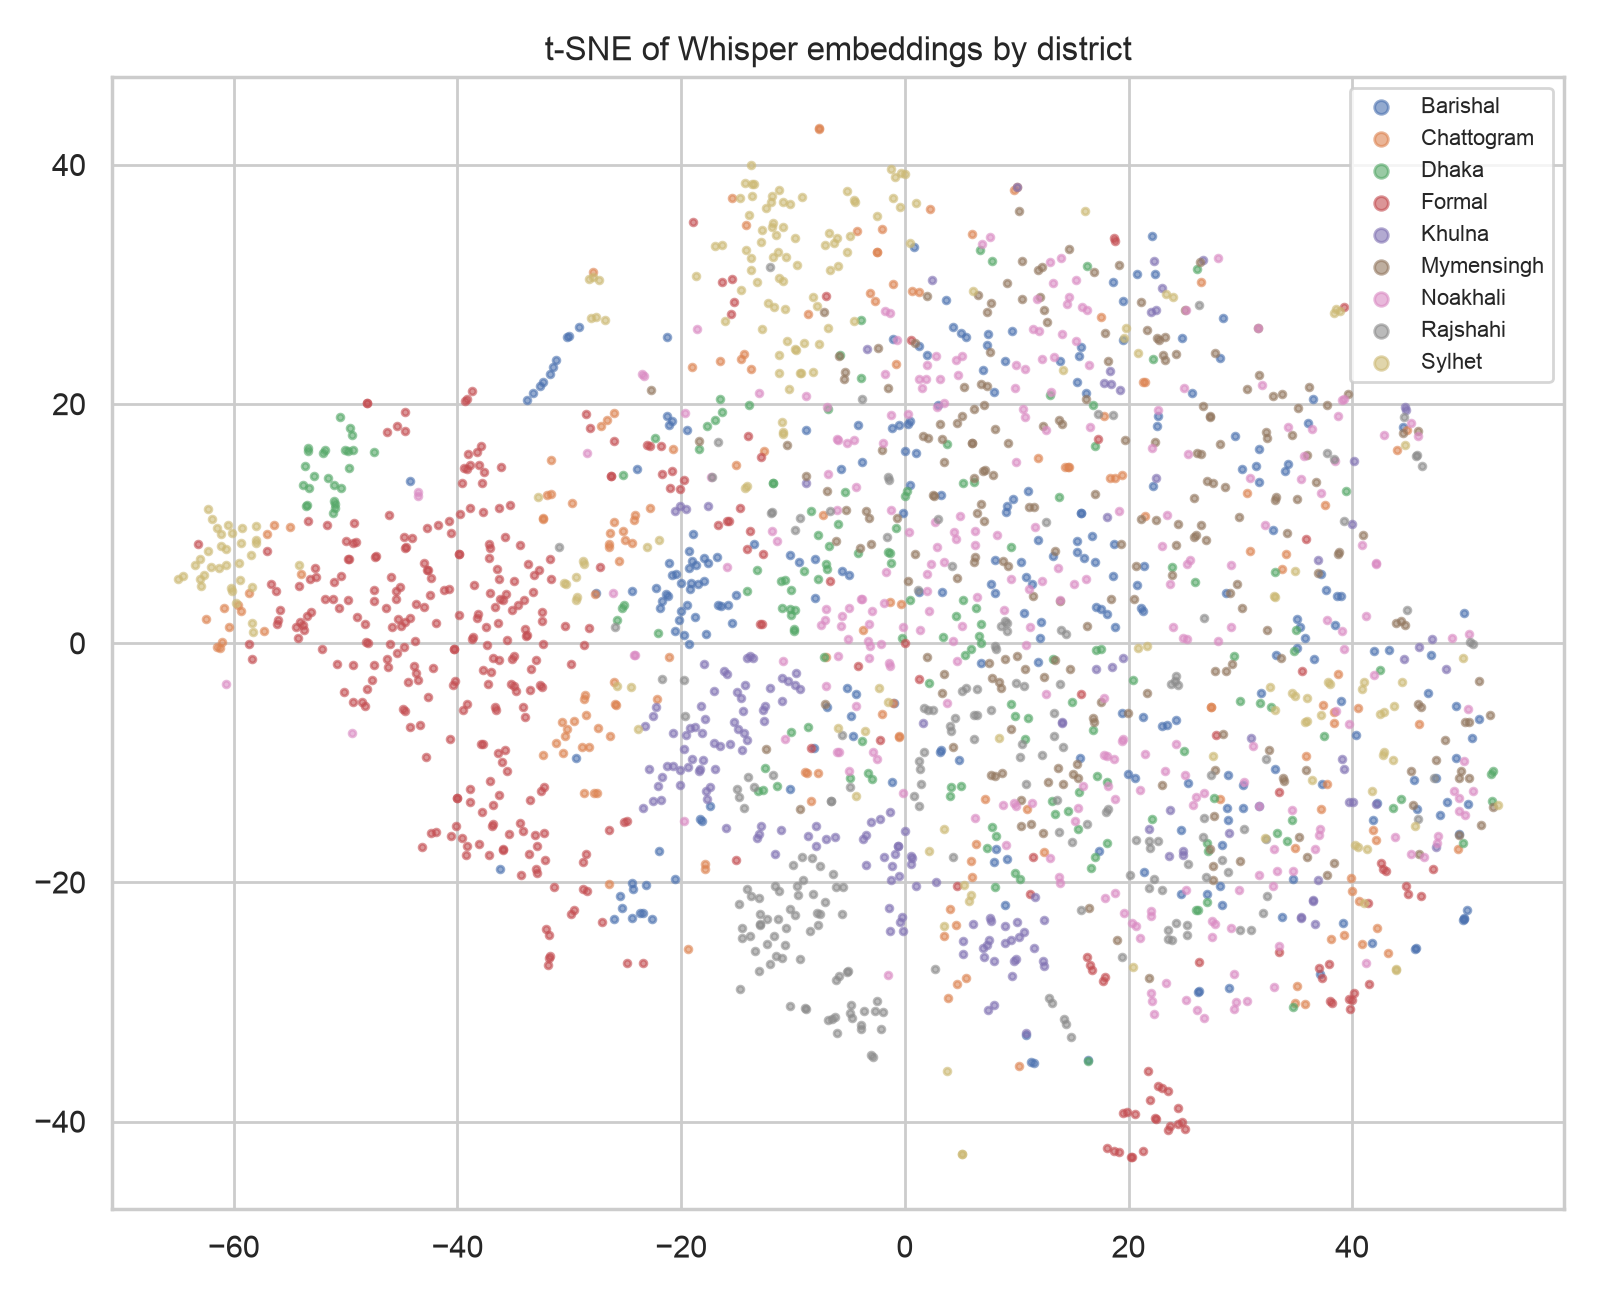
\includegraphics[width=0.7\textwidth]{tsne_embeddings.png}
  \caption{t-SNE projection of frozen Whisper-small embeddings, coloured by
  class.}
  \label{fig:tsne}
\end{figure}

\section{Strict-split results: quantifying leakage}
\label{sec:res-strict}

\Cref{tab:ablation} and \cref{fig:ablation} cross the three representations
with the two split protocols, and add the augmentation variant of
\cref{sec:method-acoustic}.

\begin{table}[ht]
  \centering
  \caption{Representation $\times$ split protocol: test macro-F1.}
  \label{tab:ablation}
  \begin{tabular}{lccc}
    \toprule
    Representation & Clip-level & Strict & $\Delta$ (points) \\
    \midrule
    MFCC statistics + MLP          & 0.727 & 0.480 & $-24.8$ \\
    Frozen Whisper-small + MLP     & 0.917 & 0.793 & $-12.4$ \\
    Fine-tuned XLS-R-300M          & 0.952 & 0.808 & $-14.4$ \\
    XLS-R-300M + channel augmentation & --- & 0.748 & --- \\
    \bottomrule
  \end{tabular}
\end{table}

\begin{figure}[ht]
  \centering
  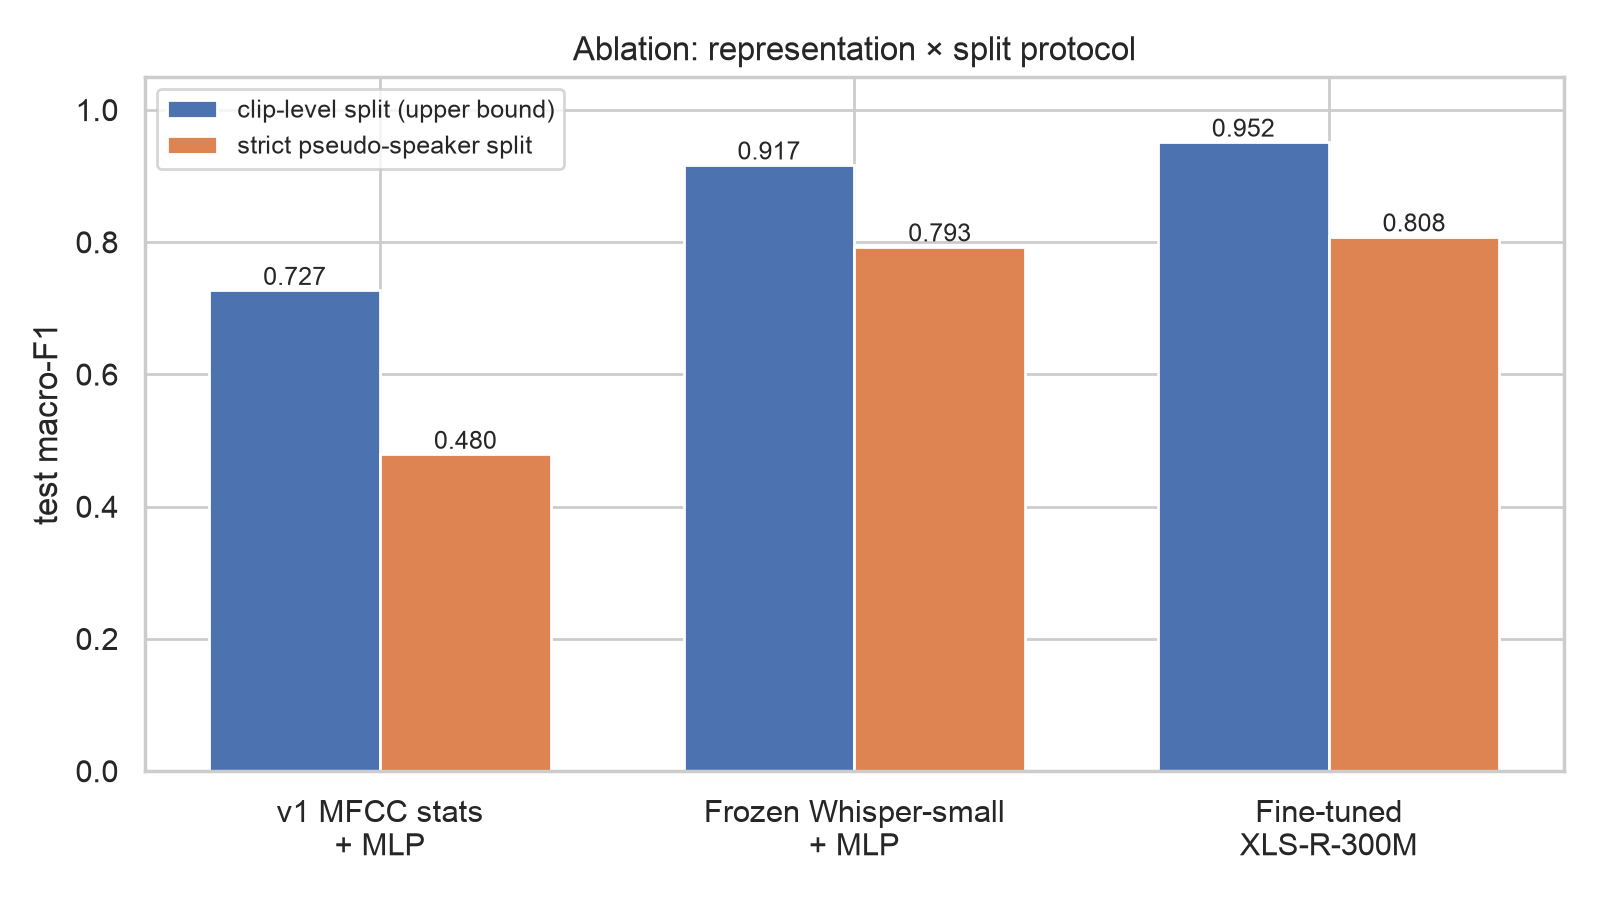
\includegraphics[width=0.85\textwidth]{ablation_representation_split.png}
  \caption{Test macro-F1 for each representation under the clip-level split
  (upper bound) and the strict pseudo-speaker split.}
  \label{fig:ablation}
\end{figure}

\begin{enumerate}
  \item \textbf{Leakage is measured at 12--14 macro-F1 points} for the
        pretrained models, and about 25 for MFCC features. The strict numbers,
        0.793 and 0.808, are the honest estimates; clip-level numbers are kept
        for comparability with prior work.
  \item \textbf{Under the strict split, fine-tuned and frozen models are
        statistically tied.} XLS-R's 1.5-point lead over frozen Whisper has a
        speaker-group bootstrap 95\,\% confidence interval of $-2.0$ to $+7.5$,
        whereas its 3.5-point clip-level lead ($+1.8$ to $+5.3$) is significant.
        Fine-tuning's strict-split drop ($-14.4$) is slightly larger than the
        frozen model's ($-12.4$).
  \item \textbf{Per-class strict scores are noisier than the macro average}
        (\cref{tab:strict-perclass}). Some strict test cells are dominated by a
        single large pseudo-speaker cluster: Barishal's strict test set is
        essentially one 251-clip cluster, so its strict F1 of 0.603 (Whisper)
        and 0.508 (XLS-R) measures generalisation to one speaker or source more
        than to the class.
\end{enumerate}

\begin{table}[ht]
  \centering
  \caption{Per-class test F1, strict split. Test sizes per class are in
  \cref{tab:classes}.}
  \label{tab:strict-perclass}
  \begin{tabular}{lccc}
    \toprule
    Class & MFCC + MLP & Frozen Whisper + MLP & Fine-tuned XLS-R \\
    \midrule
    Barishal   & 0.130 & 0.603 & 0.508 \\
    Chattogram & 0.456 & 0.670 & 0.820 \\
    Dhaka      & 0.426 & 0.881 & 0.848 \\
    Formal     & 0.694 & 0.929 & 0.785 \\
    Khulna     & 0.679 & 0.887 & 0.957 \\
    Mymensingh & 0.495 & 0.813 & 0.904 \\
    Noakhali   & 0.454 & 0.694 & 0.862 \\
    Rajshahi   & 0.372 & 0.900 & 0.842 \\
    Sylhet     & 0.611 & 0.763 & 0.750 \\
    \midrule
    Macro      & \textbf{0.480} & \textbf{0.793} & \textbf{0.808} \\
    \bottomrule
  \end{tabular}
\end{table}

The two pretrained models fail differently under the strict split: frozen
Whisper is better on Formal, Dhaka and Rajshahi, fine-tuned XLS-R on
Chattogram, Noakhali, Mymensingh and Khulna. Their macro averages are close,
but they are not the same model with different accuracy.

\paragraph{Statistical uncertainty.} \Cref{tab:ci-acoustic} gives the 95\,\%
intervals from the group bootstrap of \cref{sec:method-eval}. Clip bootstrap
intervals are narrower but understate the variance. Under the group bootstrap,
every MFCC-versus-pretrained gap is significant, as are XLS-R's clip-level lead
over Whisper and the augmentation drop ($-6.0$, interval $-9.4$ to $-0.9$);
XLS-R's strict-split lead over Whisper is not.

\begin{table}[ht]
  \centering
  \caption{Test macro-F1 with 95\,\% speaker-group bootstrap intervals
  ($B = 2{,}000$; 565 groups in the clip-level test set, 230 in the strict).}
  \label{tab:ci-acoustic}
  \begin{tabular}{lcc}
    \toprule
    Model & Clip-level & Strict \\
    \midrule
    MFCC + MLP             & 0.727 (0.676--0.753) & 0.480 (0.368--0.552) \\
    Frozen Whisper + MLP   & 0.917 (0.894--0.932) & 0.793 (0.688--0.808) \\
    Fine-tuned XLS-R       & 0.952 (0.935--0.963) & 0.808 (0.717--0.838) \\
    XLS-R + augmentation   & ---                  & 0.748 (0.649--0.792) \\
    \bottomrule
  \end{tabular}
\end{table}

\section{Data efficiency}
\label{sec:res-efficiency}

\Cref{tab:efficiency} and \cref{fig:efficiency} show test macro-F1 when the MLP
heads are trained on fractions of the training split (mean of three seeds).

\begin{table}[ht]
  \centering
  \caption{Test macro-F1 against the fraction of training data used (mean of
  three seeds).}
  \label{tab:efficiency}
  \begin{tabular}{lccccc}
    \toprule
    Fraction of training split & 10\,\% & 25\,\% & 50\,\% & 75\,\% & 100\,\% \\
    \midrule
    Whisper, clip-level & 0.788 & 0.854 & 0.902 & 0.908 & 0.913 \\
    Whisper, strict     & 0.671 & 0.751 & 0.784 & 0.790 & 0.793 \\
    MFCC, clip-level    & 0.522 & 0.618 & 0.675 & 0.707 & 0.726 \\
    MFCC, strict        & 0.371 & 0.434 & 0.475 & 0.489 & 0.494 \\
    \bottomrule
  \end{tabular}
\end{table}

\begin{figure}[ht]
  \centering
  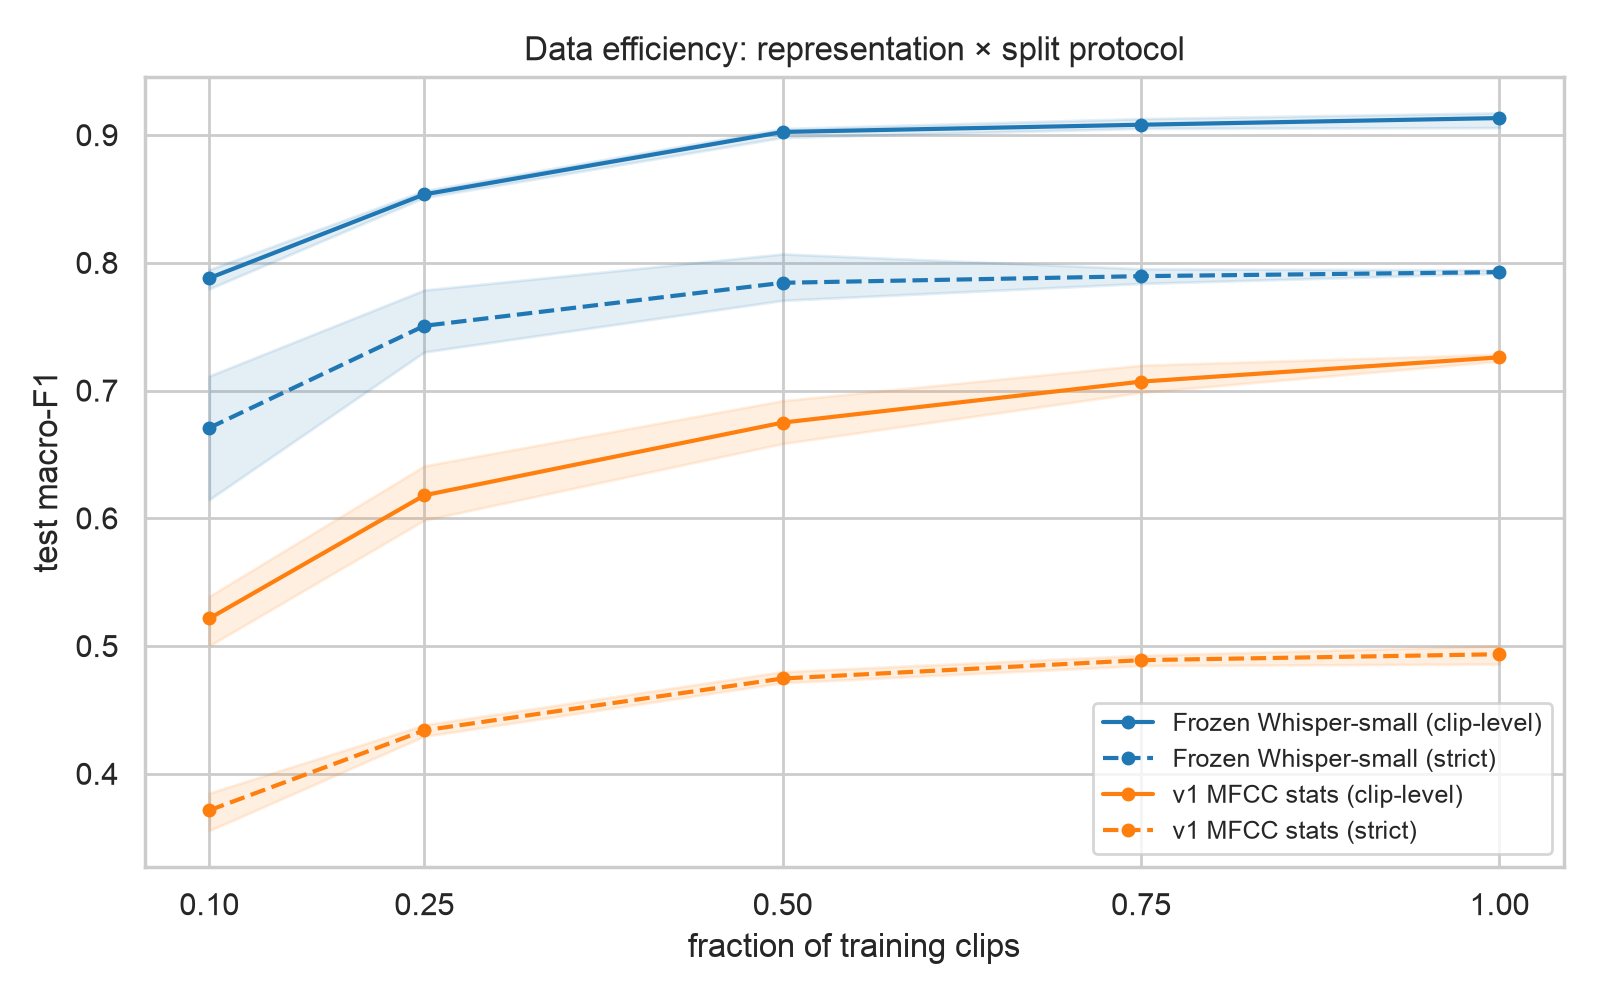
\includegraphics[width=0.85\textwidth]{data_efficiency.png}
  \caption{Data efficiency: test macro-F1 against the fraction of training clips,
  for frozen Whisper and MFCC features under both split protocols. Bands show the
  range over three seeds.}
  \label{fig:efficiency}
\end{figure}

\begin{enumerate}
  \item \textbf{Whisper embeddings trained on 10\,\% of the labels outperform MFCC
        features trained on all of them}, under both protocols. Pretraining is
        worth more than a tenfold increase in labelled data on this task.
  \item The Whisper curves flatten beyond about 50\,\%: the 13-hour corpus is
        adequately sized for the frozen-embedding approach.
  \item The gap between representations is wider under the strict split at every
        fraction, so the pretrained features' robustness to leakage holds across
        data scales.
\end{enumerate}

\section{Augmentation study}
\label{sec:res-augment}

Training the strict-split XLS-R model with the channel-suppression chain of
\cref{sec:method-acoustic} \emph{reduced} test macro-F1 from 0.808 to 0.748. The
validation score was depressed throughout training (best epoch 17 of 20,
validation 0.702 against 0.757 without augmentation), so the drop is not an
artefact of checkpoint selection. \Cref{sec:disc-augment} interprets it.

\section{The lexical route: words versus sound}
\label{sec:res-lexical}

\subsection{How much dialect survives transcription?}
\label{sec:res-asr}

\Cref{tab:asr-quality} scores the five front-ends against the human transcripts
of Ben-10's validation set, which contain 21,119 reference tokens outside the
standard vocabulary.

\begin{table}[ht]
  \centering
  \caption{Speech-recognition quality on Ben-10 validation (1,666 clips, ten
  districts; greedy decoding, punctuation ignored).}
  \label{tab:asr-quality}
  \begin{tabular}{lcccc}
    \toprule
    Front-end & WER & CER & Dialect-word recall & Formal-word recall \\
    \midrule
    Tugstugi (Ben-10)      & \textbf{0.707} & \textbf{0.471} & \textbf{0.192} & \textbf{0.455} \\
    Tugstugi               & 0.775 & 0.532 & 0.034 & 0.369 \\
    Hishab FastConformer   & 0.792 & 0.517 & 0.012 & 0.405 \\
    wav2vec2 Bengali       & 0.942 & 0.669 & 0.012 & 0.085 \\
    Whisper-large-v3       & 0.960 & 0.808 & 0.016 & 0.061 \\
    \bottomrule
  \end{tabular}
\end{table}

The ordering and size of the error rates match the Ben-10 benchmark
\citep{dipto2025ben10}, which reports 0.70 for the Ben-10-fine-tuned model on
its private test set and 0.81, 0.87 and 1.13 for Tugstugi, Hishab and
Whisper-large-v3. Even the best front-end reproduces fewer than one dialect word
in five; by district its recall ranges from 0.243 (Sylhet) to 0.135 (Rangpur).
The standard-Bangla models reproduce 1--3\,\% of dialect words. The benchmark's
hand-counted recall for the two Tugstugi models (0.16--0.53 against
0.01--0.09) is thus confirmed at full scale with an automated measure.

On the thesis corpus, which has no references, the same pattern appears in the
share of transcript words outside the standard vocabulary
(\cref{fig:asr-dialect}b). Only the Ben-10 model separates regional clips (25\,\%
on average) from Formal clips (8\,\%) by a wide margin, with recognisable dialect
forms such as \bn{mui}{মুই}, \bn{ai}{আঁই}, \bn{ar}{আঁর}, \bn{hamar}{হামার}, \bn{kita}{কিতা} and \bn{teha}{টেহা}.
Hishab and the base Tugstugi model output almost as few non-standard words on
regional clips (9\,\% and 13\,\%) as on Formal ones (4\,\% and 5\,\%). The
wav2vec~2.0 and Whisper-large-v3 front-ends have high shares for the wrong
reason: misrecognition, and for Whisper-large-v3 repetition loops in 12.3\,\% of
transcripts (one word repeated five or more times in a row) and 2.5--4.8\,\%
empty outputs per class.

\begin{figure}[ht]
  \centering
  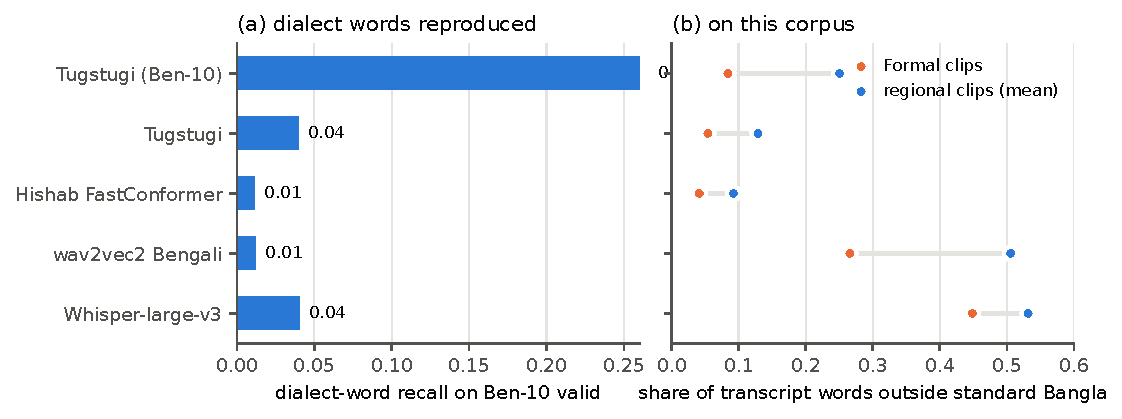
\includegraphics[width=\textwidth]{phase5_asr_dialect.pdf}
  \caption{What survives transcription. (a) Dialect-word recall of each
  front-end on Ben-10 validation. (b) Share of transcript words outside the
  standard vocabulary on this corpus, for Formal clips and the mean over the eight
  regional classes.}
  \label{fig:asr-dialect}
\end{figure}

\subsection{Classification from transcripts}

\Cref{tab:lexical} and \cref{fig:lexical} report the three classifiers for each
front-end, using the in-domain lexicon.

\begin{table}[ht]
  \centering
  \caption{Test macro-F1 of the lexical classifiers by front-end. Fine-tuned
  XLS-R alone scores 0.808 (strict) and 0.952 (clip-level).}
  \label{tab:lexical}
  \small
  \begin{tabular}{lccccc}
    \toprule
    & \multicolumn{3}{c}{Strict} & \multicolumn{2}{c}{Clip-level} \\
    \cmidrule(lr){2-4}\cmidrule(lr){5-6}
    Front-end & Word match & TF-IDF & Fusion & TF-IDF & Fusion \\
    \midrule
    Tugstugi (Ben-10)    & 0.360 & \textbf{0.633} & \textbf{0.856} & \textbf{0.728} & \textbf{0.967} \\
    Tugstugi             & 0.060 & 0.456 & 0.836 & 0.595 & 0.965 \\
    Hishab FastConformer & 0.049 & 0.445 & 0.820 & 0.553 & 0.962 \\
    wav2vec2 Bengali     & 0.077 & 0.424 & 0.825 & 0.536 & 0.960 \\
    Whisper-large-v3     & 0.156 & 0.388 & 0.800 & 0.490 & 0.954 \\
    \bottomrule
  \end{tabular}
\end{table}

\begin{figure}[ht]
  \centering
  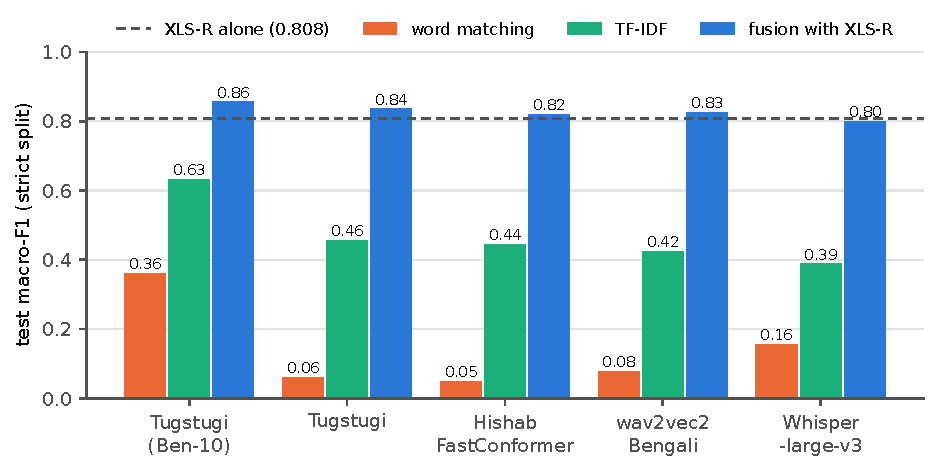
\includegraphics[width=\textwidth]{phase5_classification.pdf}
  \caption{Strict-split test macro-F1 of word matching, the TF-IDF classifier and
  fusion with XLS-R, by speech-recognition front-end. The dashed line is XLS-R
  alone.}
  \label{fig:lexical}
\end{figure}

\begin{enumerate}
  \item \textbf{Word matching is weak} even with the best front-end: 0.360
        strict and 0.399 clip-level. Fewer than half of the strict test clips
        (44\,\%) contain any lexicon word, so the rest default to Formal.
        Relaxing the lexicon thresholds raises coverage to 59\,\% and macro-F1
        to 0.419, still far below every pretrained acoustic model. The clean
        external lexicon (Ben-10 and Vashantor; six classes including Formal)
        scores 0.418 on its own classes with 51\,\% coverage. With the
        standard-Bangla front-ends, coverage collapses to 2--5\,\% and matching
        fails: there are no regional words left to match.
  \item \textbf{The TF-IDF classifier roughly doubles the matching score}
        (0.633 strict with the Ben-10 model), placing the words alone between
        MFCC features (0.480) and frozen Whisper (0.793). The front-ends rank
        exactly as their word error rates on Ben-10 do
        (\cref{tab:asr-quality}).
  \item \textbf{Fusion improves on XLS-R with four of the five front-ends.} With
        the Ben-10 model the strict score rises from 0.808 to 0.856
        ($\alpha = 0.25$, so after tuning the text carries three quarters of the
        log-probability weight) and the clip-level score from 0.952 to 0.967
        ($\alpha = 0.30$).
\end{enumerate}

\subsection{Statistical uncertainty}

\Cref{tab:ci-lexical} gives intervals for the Ben-10 front-end, and
\cref{tab:fusion-gains} the fusion gain over XLS-R for every front-end.

\begin{table}[ht]
  \centering
  \caption{Lexical-route test macro-F1 with 95\,\% speaker-group bootstrap
  intervals (Ben-10 front-end).}
  \label{tab:ci-lexical}
  \begin{tabular}{lcc}
    \toprule
    Model & Clip-level & Strict \\
    \midrule
    Word matching          & 0.399 (0.359--0.421) & 0.360 (0.284--0.380) \\
    TF-IDF                 & 0.728 (0.684--0.748) & 0.633 (0.538--0.642) \\
    Fusion XLS-R + TF-IDF  & 0.967 (0.952--0.976) & 0.856 (0.754--0.875) \\
    Fine-tuned XLS-R (reference) & 0.952 (0.935--0.963) & 0.808 (0.717--0.838) \\
    \bottomrule
  \end{tabular}
\end{table}

\begin{table}[ht]
  \centering
  \caption{Fusion gain over XLS-R alone in macro-F1 points, with 95\,\%
  speaker-group bootstrap interval and the bootstrap probability of no gain.}
  \label{tab:fusion-gains}
  \small
  \begin{tabular}{lcccc}
    \toprule
    & \multicolumn{2}{c}{Clip-level} & \multicolumn{2}{c}{Strict} \\
    \cmidrule(lr){2-3}\cmidrule(lr){4-5}
    Front-end & Gain (CI) & $P(\le 0)$ & Gain (CI) & $P(\le 0)$ \\
    \midrule
    Tugstugi (Ben-10)    & $+1.5$ ($+0.9$, $+2.4$) & 0.000 & $+4.8$ ($-0.3$, $+6.8$) & 0.04 \\
    Tugstugi             & $+1.3$ ($+0.5$, $+2.2$) & 0.002 & $+2.7$ ($-1.0$, $+4.2$) & 0.20 \\
    Hishab FastConformer & $+1.0$ ($+0.4$, $+1.7$) & 0.001 & $+1.1$ ($-2.0$, $+2.2$) & 0.39 \\
    wav2vec2 Bengali     & $+0.8$ ($+0.1$, $+1.7$) & 0.015 & $+1.7$ ($-0.2$, $+3.1$) & 0.04 \\
    Whisper-large-v3     & $+0.2$ ($-0.7$, $+1.1$) & 0.32  & $-0.8$ ($-3.8$, $+0.6$) & 0.90 \\
    \bottomrule
  \end{tabular}
\end{table}

At clip level the fusion gain is significant for every front-end except
Whisper-large-v3. Under the strict split no interval excludes zero; the Ben-10
and wav2vec~2.0 front-ends come closest (a 4\,\% bootstrap probability of no
gain), and with Whisper-large-v3 fusion is slightly worse than XLS-R alone.

\subsection{Where the words help}

\Cref{tab:fusion-perclass} and \cref{fig:fusion-perclass} break the strict-split
result down by class for the Ben-10 front-end.

\begin{table}[ht]
  \centering
  \caption{Per-class test F1, strict split, Ben-10 front-end.}
  \label{tab:fusion-perclass}
  \begin{tabular}{lccccc}
    \toprule
    Class & Word match & TF-IDF & XLS-R & Fusion & $\Delta$ fusion $-$ XLS-R \\
    \midrule
    Barishal   & 0.268 & 0.544 & 0.508 & 0.720 & $\mathbf{+21.2}$ \\
    Sylhet     & 0.600 & 0.750 & 0.750 & 0.832 & $+8.2$ \\
    Chattogram & 0.392 & 0.617 & 0.820 & 0.878 & $+5.8$ \\
    Formal     & 0.448 & 0.805 & 0.785 & 0.835 & $+5.0$ \\
    Noakhali   & 0.500 & 0.707 & 0.862 & 0.898 & $+3.5$ \\
    Mymensingh & 0.395 & 0.694 & 0.904 & 0.928 & $+2.4$ \\
    Rajshahi   & 0.175 & 0.550 & 0.842 & 0.857 & $+1.5$ \\
    Dhaka      & 0.158 & 0.470 & 0.848 & 0.853 & $+0.5$ \\
    Khulna     & 0.305 & 0.557 & 0.957 & 0.904 & $-5.3$ \\
    \bottomrule
  \end{tabular}
\end{table}

\begin{figure}[ht]
  \centering
  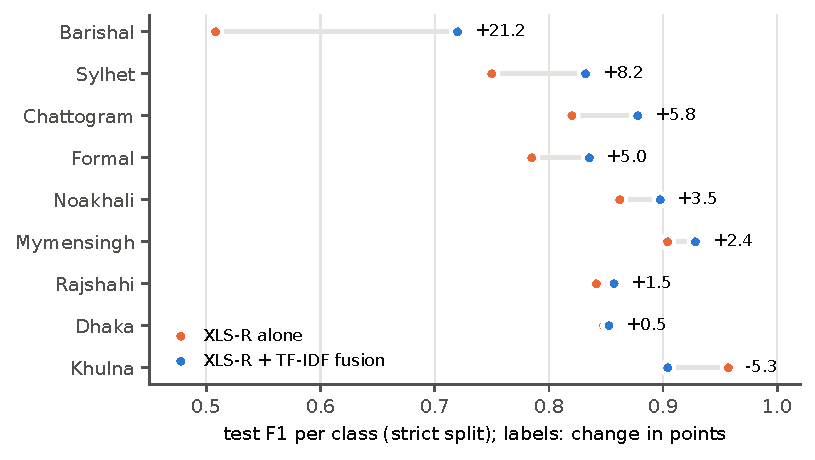
\includegraphics[width=0.8\textwidth]{phase5_fusion_per_class.pdf}
  \caption{Per-class test F1 on the strict split for XLS-R alone and for its
  fusion with the TF-IDF transcript classifier (Ben-10 front-end). Labels give
  the change in F1 points.}
  \label{fig:fusion-perclass}
\end{figure}

The gain concentrates on the classes the acoustic model finds hardest under the
strict split---Barishal, the single-cluster test cell, and Sylhet---and on the
classes with the most distinctive, best-transcribed vocabulary: Sylhet's match
F1 of 0.600 is the only strong word-matching result. Khulna, the acoustic
model's best class, is the one class that fusion hurts. Formal is the only class
on which the text classifier alone beats XLS-R: the standard register is marked
in its vocabulary.

\chapter{Discussion}
\label{ch:discussion}

\section{What the strict split reveals}
\label{sec:disc-strict}

The central methodological result is that a disclaimer became a measurement.
Most audio classification on found data either ignores speaker and channel
leakage or mentions it qualitatively. Here the pseudo-speaker split bounds it:
12--14 macro-F1 points for pretrained representations and about 25 for
hand-crafted features. Three implications follow.

\begin{enumerate}
  \item \textbf{Scores reported on clip-level splits of found-data corpora are
        inflated, and by an amount that depends on the representation.}
        Comparing papers that use different features on clip-level splits
        partly ranks how well each exploits the channel, not how well it
        identifies dialect.
  \item \textbf{The honest acoustic headline for this corpus is 0.808}
        (fine-tuned XLS-R, strict split). That remains a strong 9-way result,
        about seven times chance, on speakers the model has never heard.
  \item \textbf{Per-class strict numbers must be read with care.} Barishal's
        strict test set is a single 251-clip pseudo-speaker cluster, so its fall
        from 0.871 to 0.603 for the frozen model measures generalisation to one
        speaker or source rather than to the class. Conclusions at the macro
        level are the robust ones.
\end{enumerate}

\section{Errors follow dialect geography}
\label{sec:disc-geography}

Under every model and protocol the dominant confusion is between Barishal and
Noakhali, two southern coastal dialects with documented linguistic proximity,
and Mymensingh, a transitional zone, spreads its errors across its neighbours.
This is linguistically coherent behaviour: the models' mistakes recapitulate the
dialect continuum rather than arbitrary decision boundaries, which supports the
claim that they learn accentual structure and not only channel shortcuts, even
on the clip-level split.

\section{The shrinking advantage of fine-tuning}
\label{sec:disc-finetune}

Fine-tuned XLS-R gains 3.5 points over frozen Whisper at clip level, a
significant difference, but only 1.5 under the strict split, which is not
significant, and its strict-split drop ($-14.4$) is slightly larger than the
frozen model's ($-12.4$). End-to-end adaptation lets a model exploit whatever
separates the training classes, including channel signatures that correlate with
class in the training data; a frozen, general-purpose representation cannot
specialise in this way. The practical lesson is that, when leakage cannot be
ruled out, frozen-embedding baselines are not merely cheaper: they partly
protect against shortcut learning, and a fine-tuning margin measured on a leaky
split overstates the improvement that would hold in deployment. The comparison
is confounded, however: the frozen model is Whisper-small and the fine-tuned one
XLS-R-300M, so ``frozen versus fine-tuned'' and ``Whisper versus XLS-R'' are not
separated (\cref{sec:disc-limits}).

\section{The augmentation result: prosody is signal}
\label{sec:disc-augment}

The channel-suppression chain lowered strict-split macro-F1 by six points. The
chain included pitch shift ($\pm 2$ semitones) and time stretch (0.9--1.1),
transforms that are standard and beneficial in speech recognition
\citep{ko2015augmentation}, where the transcript is invariant to prosody.
Dialect identification inverts this: pitch contour, rhythm and tempo carry
dialect, so these transforms corrupt the evidence for the label rather than
removing nuisance variation. Probing work showing that accent fine-tuning
reshapes prosodic encoding in wav2vec~2.0 \citep{yang2023accent} supports this
reading, and the validation score, depressed throughout training (0.702 against
0.757), indicates a harder target rather than an unlucky checkpoint.

The recommendation is task-specific: augmentation for dialect and accent
identification should preserve prosody (additive noise, equalisation, band
limiting, gain), and prosodic perturbation should be treated as harmful until
shown otherwise. The reduced chain was not tested and is left as future work;
without that test, the attribution to the pitch and tempo transforms remains a
hypothesis.

\section{Words or sound?}
\label{sec:disc-words}

The lexical route reads the thesis title literally: how much of Bangla dialect
identity is in the words, and how much lies beyond them? Three findings stand
out.

\paragraph{Standard-Bangla speech recognition removes the dialect before a
classifier can see it.} Recognisers trained on standard Bangla (Tugstugi,
Hishab) transcribe regional speech into standard forms---\bn{biya}{বিয়া দিয়া দাও}
(``arrange the marriage'') becomes \bn{biye}{বিয়ে দিয়ে দাও}---and reproduce only
1--3\,\% of the dialect words in Ben-10's human transcripts. Their output on
regional clips is barely less standard than on Formal clips. The one front-end
fine-tuned on dialect speech reproduces 19\,\%, which is both the best available
and a hard ceiling for any word-list method: four of five dialect words never
reach the text. This confirms, with an automated measure over the full
validation set, the observation that \citet{dipto2025ben10} made by hand, and it
is the single most important fact about the lexical route.

\paragraph{Filtering to regional words discards evidence.} The intuitive
design---drop every word that standard Bangla also has and match what is left
against regional word lists---scores 0.360 under the strict split, because
fewer than half of the 5-second clips keep any matchable word. A TF-IDF
classifier over all words and character n-grams reaches 0.633 on the same
transcripts. Two mechanisms plausibly explain the gap, though this thesis did
not isolate them: words that also exist in standard Bangla but are used at
different rates across regions (pronouns, particles, common verbs), which the
filter removes; and character n-grams, which generalise over rare inflected
dialect forms such as verb endings that never reach the lexicon's frequency
thresholds. Word matching keeps its value as an \emph{explanation}---it shows
which words decided a clip and how strongly each belongs to each region---rather
than as the classifier.

\paragraph{Words and sound are complementary, modestly.} Fusion raises the
honest headline from 0.808 to 0.856, a gain that is borderline under the
speaker-group bootstrap (a 4\,\% probability of no gain), and the clip-level
score from 0.952 to 0.967, which is significant. The gain lands where the
acoustic model is weakest under the strict split---Barishal (+21 points) and
Sylhet (+8), the dialect with the most distinctive and best-transcribed
vocabulary---and is negative only for Khulna, where the acoustics are already
near perfect. The two routes fail on different clips, which is the condition
under which fusion helps, and this is evidence that the text carries dialect
information of its own rather than a noisier copy of the acoustic decision.

\paragraph{The answer.} For clips this short, dialect identity lies
\emph{mostly beyond the words}. Words alone (0.633) sit between hand-crafted
acoustics (0.480) and frozen Whisper (0.793); the acoustic route is the stronger
single route, and the lexical route's ceiling is set by speech recognition, not
by the classifier. Two caveats temper the comparison. The TF-IDF model may
partly learn programme- or topic-specific vocabulary, because the strict split
separates speakers but not content, so 0.633 is itself an upper bound on the
dialect information in the words. And the acoustic models were trained on 13
hours of in-domain audio, whereas the recognisers saw none of it: a
dialect-aware recogniser trained on this corpus would raise the lexical ceiling,
at the cost of the off-the-shelf setting that makes the comparison clean.

\section{Limitations}
\label{sec:disc-limits}

\begin{itemize}
  \item \textbf{Pseudo-speakers are approximate.} Calibration against Formal's
        true sources reaches an ARI of 0.347, and clustering both over-merges (a
        251-clip Barishal cluster) and over-splits (many singletons). The strict
        split removes much, but not provably all, speaker and channel overlap;
        true speaker labels would tighten the estimate in both directions.
  \item \textbf{Uneven strict test cells.} Group-disjoint splitting with
        unequal clusters concentrates some classes' test sets in a few clusters,
        so per-class strict numbers have high variance.
  \item \textbf{Short clips.} Five seconds excludes longer-range dialect cues
        such as discourse markers and phrase-level intonation.
  \item \textbf{Single domain.} The corpus is broadcast and online media;
        generalisation to conversational or telephone speech is untested.
  \item \textbf{Model family is confounded with adaptation regime.} The frozen
        model is Whisper-small and the fine-tuned one XLS-R-300M. Frozen XLS-R
        embeddings, cheap to compute locally, would separate the two factors.
  \item \textbf{Single-seed fine-tuning.} Each XLS-R result is one seed; the
        bootstrap intervals cover test-set sampling noise, not training-seed
        variance.
  \item \textbf{Whisper pooling includes padding.} Whisper's encoder always
        processes 30\,s of input, and the baseline mean-pools all 1,500 frames,
        of which only about 250 cover the 5\,s of speech. The padding
        contribution is the same for every clip, but pooling only speech frames
        would be the cleaner design.
  \item \textbf{Authenticity of found data.} Clips from films and dramas may
        include actors performing a dialect rather than native speakers.
  \item \textbf{No reference transcripts for the corpus.} Recognition quality is
        measured on Ben-10, a different corpus with longer, spontaneous clips
        and only three districts in common; word error rate on this corpus is
        unknown. Hand-transcribing a subset of about 20 clips per class would
        close this gap.
  \item \textbf{Content leakage is not controlled.} The strict split is
        speaker-disjoint, not topic-disjoint; recurring programmes, names and
        topics can appear on both sides and inflate the text classifier. The
        in-domain lexicon's two-speaker rule and the external lexicon mitigate,
        but do not remove, this risk.
  \item \textbf{Front-end substitutions.} The benchmark's ``Wav2Vec2 (SCB)''
        checkpoint is not public, and the wav2vec~2.0 model used instead is a
        different model; Google's recogniser and the benchmark's Ben-10-tuned
        wav2vec~2.0 were not run. The Ben-10-tuned recogniser was trained on ten
        districts, of which only Barishal, Chattogram and Sylhet are classes
        here, and Khulna, Rajshahi and Dhaka have no clean external word list.
  \item \textbf{Validation reuse.} The XLS-R checkpoint was selected on the same
        validation split later used to tune the fusion weight $\alpha$, so
        XLS-R's validation probabilities are mildly optimistic and $\alpha$ may
        lean towards the acoustic model. Test numbers are unaffected, and all
        tuning used validation data only.
  \item \textbf{Greedy, single decoding.} Each front-end's transcripts are one
        greedy decode; beam search or temperature fallback might reduce
        Whisper-large-v3's repetition loops.
\end{itemize}

\section{Future work}
\label{sec:disc-future}

\begin{itemize}
  \item A prosody-preserving augmentation chain on the strict split, the direct
        test of \cref{sec:disc-augment}.
  \item True speaker annotation for a subset, to validate the pseudo-speaker
        estimate.
  \item Larger multilingual encoders (XLS-R-1B, MMS) within the same free-GPU
        budget, and frozen XLS-R embeddings to remove the model-family confound.
  \item Longer inputs, and aggregation of clip decisions to speaker or
        recording level.
  \item Cross-domain evaluation on conversational and telephone speech.
  \item For the lexical route: a dialect-aware recogniser fine-tuned on this
        corpus, since transcription rather than classification is the
        bottleneck; a hand-transcribed subset for word error rate on this
        corpus; a topic-disjoint split to bound content leakage; and joint
        rather than late fusion, feeding text features into the acoustic model.
\end{itemize}

\chapter{Conclusion}
\label{ch:conclusion}

This thesis set out to identify nine Bangla dialect classes from 5-second clips
of found media, to measure how much of the apparent accuracy comes from
recognising speakers and recording channels, and to ask whether dialect identity
is carried by the sound or by the words. The answers to the four research
questions are as follows.

\paragraph{RQ1: accuracy of pretrained speech models.} Pretrained models far
outperform hand-crafted features. On a conventional clip-level split, frozen
Whisper-small embeddings reach a macro-F1 of 0.917 and fine-tuned XLS-R-300M
0.952, against 0.727 for MFCC statistics. Frozen Whisper embeddings trained on
10\,\% of the labels outperform MFCC features trained on all of them.

\paragraph{RQ2: the effect of leakage.} A strict split built from ECAPA-TDNN
pseudo-speaker clusters, calibrated against the known sources of the Formal
clips, lowers the pretrained models to 0.793 and 0.808: 12--14 points of their
clip-level scores came from speaker and channel overlap. The ranking of
pretrained over hand-crafted features survives, but fine-tuning's advantage over
frozen embeddings does not reach significance, and channel-suppression
augmentation that perturbs pitch and tempo lowers the score to 0.748.

\paragraph{RQ3: dialect information in the words.} Off-the-shelf Bangla speech
recognition loses most of it. The best recogniser, fine-tuned on regional speech
by its publishers, reproduces 19\,\% of dialect words in human transcripts;
recognisers trained on standard Bangla reproduce 1--3\,\%, rewriting dialect
into the standard form. Matching regional word lists therefore identifies the
dialect poorly (0.360 under the strict split), and a text classifier over the
full transcript reaches 0.633---between hand-crafted and pretrained acoustics.

\paragraph{RQ4: complementarity.} The routes are complementary, modestly.
Combining the text classifier with the acoustic model raises the strict-split
score from 0.808 to 0.856 (borderline under the speaker-group bootstrap) and the
clip-level score from 0.952 to 0.967 (significant). The gain is largest on the
classes the acoustic model finds hardest.

\medskip
The overall conclusion is that, on clips this short, Bangla dialect identity lies
mostly \emph{beyond the words}: in pronunciation, rhythm and intonation that
pretrained speech models capture and that speech recognition trained on the
standard language discards. The honest headline for this corpus is 0.808 from
sound alone and 0.856 with words added, on speakers the models have never heard.
Two practical lessons extend beyond Bangla: dialect and accent scores on found
data should be reported under a speaker-disjoint protocol, because the
clip-level numbers flatter every model and some more than others; and text-based
dialect methods built on speech recognition are limited by how much dialect the
recogniser preserves, which should be measured before the classifier is built.

All code, split files, transcripts, word lists and per-clip predictions are
released, and \cref{app:repro} maps every number in this thesis to the command
that produces it.


% ---------- Back matter -----------------------------------------------
\cleardoublepage
\phantomsection
\addcontentsline{toc}{chapter}{Bibliography}
\bibliography{references}

\appendix
\chapter{Reproducibility}
\label{app:repro}

Every result maps to one command in the code repository, run at seed 42 on the
committed split files \path{splits/manifest_split_rel.csv} (clip-level) and
\path{splits/manifest_split_strict_rel.csv} (strict). Relative paths in the
split files resolve against the audio root, which is not redistributed.

\section{Environment}

\begin{itemize}
  \item \textbf{Local:} Python 3.12, \path{pip install -r requirements.txt}.
        PyTorch selects CUDA, then Apple MPS, then CPU. MLP heads are trained on
        CPU for bit-reproducibility.
  \item \textbf{Cloud:} Kaggle T4 GPU for fine-tuning and transcription
        (\path{kaggle kernels push --accelerator NvidiaTeslaT4}; Kaggle's
        default P100 assignment is not supported by current PyTorch builds).
\end{itemize}

\section{Acoustic route}

\begin{small}
\noindent\begin{tabularx}{\textwidth}{@{}>{\raggedright\arraybackslash}p{4.2cm}L@{}}
  \toprule
  Result & Command \\
  \midrule
  Whisper clip-level 0.917 & \path{baseline_whisper.py cache}, then \path{baseline_whisper.py train --device cpu} \\
  Whisper strict 0.793 & same, with \path{--remap-split manifest_split_strict.csv} \\
  MFCC clip-level 0.727 & \path{baseline_mfcc.py cache}, then \path{baseline_whisper.py train --emb features_v1.npz --device cpu} \\
  MFCC strict 0.480 & same, with \path{--remap-split manifest_split_strict.csv} \\
  XLS-R clip-level 0.952 & \path{finetune_xlsr.py --manifest splits/manifest_split_rel.csv} (T4, 20 epochs) \\
  XLS-R strict 0.808 & \path{finetune_xlsr.py --manifest splits/manifest_split_strict_rel.csv} (T4, 20 epochs) \\
  XLS-R strict + augmentation 0.748 & same, with \path{--augment} \\
  Data efficiency & \path{data_efficiency.py} \\
  Bootstrap intervals & \path{bootstrap_ci.py} $\rightarrow$ \path{reports/phase3/bootstrap_ci.json} \\
  \bottomrule
\end{tabularx}
\end{small}

\section{Lexical route}

External inputs (not redistributed): OOD-Speech \path{train.csv} (Kaggle
competition \path{bengaliai-speech}), Ben-10 training and validation CSVs and
validation audio (Hugging Face \path{bengaliAI/Ben-10}), and the Vashantor CSV
release (Mendeley Data).

\begin{small}
\noindent\begin{tabularx}{\textwidth}{@{}>{\raggedright\arraybackslash}p{4.2cm}L@{}}
  \toprule
  Result & Command \\
  \midrule
  Transcripts (9,303 clips $\times$ 5 front-ends) & \path{notebooks/kaggle_transcribe.ipynb}, wrapping \path{transcribe.py} $\rightarrow$ \path{transcripts/<front-end>.csv} \\
  Standard vocabulary & \path{build_lexicon.py formal --source data/ood_speech/train.csv} \\
  External lexicon & \path{build_lexicon.py external --ben10 data/ben10/train.csv --vashantor data/vashantor/Vashantor_CSV_Format} \\
  In-domain lexicons & \path{build_lexicon.py indomain --transcripts transcripts/<front-end>.csv --manifest splits/<split>.csv} \\
  XLS-R probabilities for fusion & \path{predict.py --checkpoint checkpoints/xlsr_strict_best.pt --manifest splits/manifest_split_strict_rel.csv --dump-probs reports/phase5/xlsr_probs_strict.csv} \\
  Word matching, TF-IDF, fusion & \path{lexical_did.py --transcripts ... --lexicon ... --xlsr-probs ...} $\rightarrow$ \path{reports/phase5/metrics_*.json} \\
  Front-end diagnostics & \path{asr_diagnostics.py transcripts/<front-end>.csv --min-count 3} \\
  Recognition quality on Ben-10 & \path{notebooks/kaggle_ben10_eval.ipynb}, then \path{ben10_eval.py transcripts/ben10_valid/*.csv} \\
  Summary table and figures & \path{summarize_phase5.py}, \path{make_phase5_figures.py} \\
  Bootstrap intervals & \path{bootstrap_ci.py --extra "strict:Fusion/...=..."} $\rightarrow$ \path{reports/phase5/bootstrap_ci.json} \\
  \bottomrule
\end{tabularx}
\end{small}

\section{Determinism}

MLP-head results are bit-reproducible on CPU at seed 42; MPS and CUDA runs land
within $\pm 0.005$ macro-F1. Fine-tuning on a T4 in fp16 is reproducible at the
reported precision (cuDNN non-determinism affects the fourth decimal). Embedding
and feature caches are deterministic given the manifest order. Greedy
transcripts on a T4 (fp16) and on an M1 (fp32) agree on 93.6\,\% of a 450-clip
pilot; the reported numbers use the T4 transcripts.

\chapter{Settings Reference}
\label{app:settings}

\begin{table}[ht]
  \centering
  \caption{Training and evaluation settings.}
  \label{tab:settings}
  \small
  \begin{tabularx}{\textwidth}{@{}lL@{}}
    \toprule
    Setting & Value \\
    \midrule
    \multicolumn{2}{@{}l}{\textit{Shared}} \\
    Seed & 42 \\
    Loss & cross-entropy with inverse-frequency class weights \\
    Model selection & best validation macro-F1 \\
    Bootstrap & $B = 2{,}000$; clip and pseudo-speaker-group resampling; 95\,\% percentile intervals \\
    \midrule
    \multicolumn{2}{@{}l}{\textit{MLP head (MFCC and frozen Whisper)}} \\
    Architecture & input--256--256--9, ReLU, dropout 0.3 \\
    Optimiser & AdamW, learning rate $10^{-3}$, weight decay $10^{-4}$ \\
    Schedule & 60 full-batch epochs on CPU \\
    MFCC features & 40 MFCC + $\Delta$ + $\Delta\Delta$, mean and s.d.\ pooled (240-d) \\
    Whisper features & \hf{openai/whisper-small} encoder, mean-pooled (768-d) \\
    \midrule
    \multicolumn{2}{@{}l}{\textit{Fine-tuned XLS-R}} \\
    Model & \hf{facebook/wav2vec2-xls-r-300m}, convolutional encoder frozen \\
    Learning rates & encoder $2\times10^{-5}$, head $10^{-4}$; 10\,\% warm-up, linear decay \\
    Batch & 8 $\times$ 2 accumulation (effective 16), fp16, gradient clip 1.0 \\
    Epochs & 20 \\
    Input & 5\,s waveform, padded or trimmed, per-utterance normalised \\
    \midrule
    \multicolumn{2}{@{}l}{\textit{Strict split}} \\
    Speaker embeddings & \hf{speechbrain/spkrec-ecapa-voxceleb} (192-d) \\
    Clustering & agglomerative, cosine distance, average linkage, threshold 0.50 (ARI 0.347 on Formal sources) \\
    \midrule
    \multicolumn{2}{@{}l}{\textit{Lexical route}} \\
    Decoding & greedy; Whisper: language and task fixed to Bangla transcription, $\le$128 new tokens (5\,s clips) or $\le$440 (Ben-10 valid); CTC: arg\,max, no language model \\
    Standard vocabulary & OOD-Speech training sentences, word types with count $\ge 3$ (88,262) \\
    In-domain lexicon & training split only; count $\ge 3$ in $\ge 2$ pseudo-speakers; add-$\tfrac12$ smoothing \\
    Word matching & Formal threshold $\tau$ tuned on validation, grid 0.00--0.50 in steps of 0.02 \\
    TF-IDF & word 1--2-grams + character 2--5-grams, sublinear TF, min.\ document frequency 2 \\
    Logistic regression & balanced class weights, $C \in \{0.3, 1, 3, 10, 30\}$ tuned on validation \\
    Fusion & $\alpha \in \{0, 0.05, \dots, 1\}$ tuned on validation \\
    \bottomrule
  \end{tabularx}
\end{table}

\chapter{Additional Figures}
\label{app:figures}

\begin{figure}[ht]
  \centering
  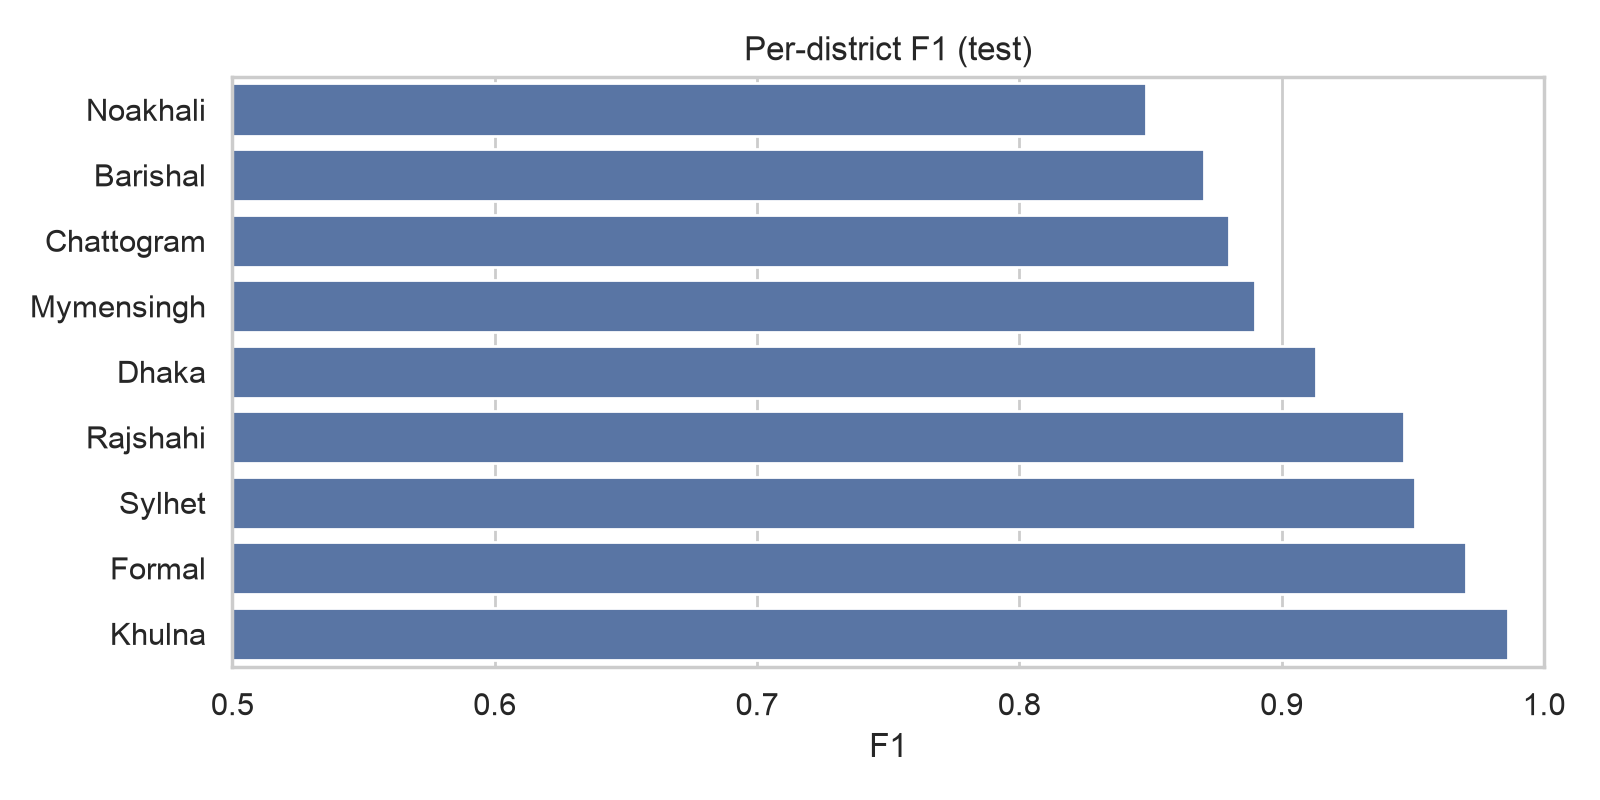
\includegraphics[width=0.85\textwidth]{per_class_f1_baseline.png}
  \caption{Per-class test F1 of the frozen Whisper-small baseline on the
  clip-level split (macro-F1 0.917), sorted by score. The same values appear in
  \cref{tab:clip-perclass} and \cref{fig:perclass-clip}.}
  \label{fig:perclass-baseline}
\end{figure}


\end{document}
